\documentclass[a4paper,11pt]{article}
\usepackage[T1]{fontenc}		% codifica dei font
\usepackage[utf8]{inputenc}  	% lettere accentate da tastiera
\usepackage[italian]{babel}  	% lingua del documento
\usepackage[italian]{isodate}  	% formato delle date in italiano
\usepackage{graphicx}			% gestione pdf come immagini
\usepackage{pifont}				% stili per gli elenchi puntati
\usepackage{enumitem}

\usepackage{xcolor}

\usepackage[linkcolor=black, citecolor=blue, urlcolor=cyan]{hyperref}
\hypersetup{
	colorlinks=true
}

\renewcommand\labelitemi{--}

% Comandi personalizzati
\newcommand{\SP}{\mbox{ }}
\renewcommand{\arraystretch}{2}
\renewcommand{\labelenumii}{\theenumii}
\renewcommand{\theenumii}{\theenumi.\arabic{enumii}.}


\begin{document}

\title{Documentazione progetto Ingegneria del software}
\author{VR458509\\VR460035\\VR443470}
\date{\printdayoff\today}	% eliminazione del giorno dalla data
\maketitle

\newpage

\tableofcontents	% indice
	
\newpage
%%%%%%%%%%%%%%%%%%%%%%%%%%%%%%%%%%%%%%%%%%%%%%%%
%%%%%%%%%%% INGEGNERIA DEI REQUISITI %%%%%%%%%%%
%%%%%%%%%%%%%%%%%%%%%%%%%%%%%%%%%%%%%%%%%%%%%%%%
\section{Ingegneria dei requisiti}
\label{pri:ing_req}
I requisiti forniti al team di sviluppo, mediante testo, sono stati minuziosamente analizzati e successivamente raffinati tramite interviste chiuse (via e-mail) con il cliente. Il passo iniziale quindi, è stato quello di ottenere i diagrammi UML (\emph{usecase and activity diagram}).\\
\\
I passi successivi sono stati:
\begin{enumerate}
	\item Stilare i requisiti come una lista di compiti (\emph{task}) da eseguire;
	\item Eseguire una stima del tempo richiesto per completare ciascun\SP elemento;
	\item Assegnare ciascun \emph{task} ad ogni sviluppatore.
\end{enumerate}
Le metodologie di sviluppo utilizzate verranno introdotte nei paragrafi successivi.\\
\\
Sono stati creati vari prototipi con l'obbiettivo di essere presentati al cliente e di ottenere una convalida dei requisiti dedotti dal testo. Ogni prototipo ha dunque consentito di migliorare la specifica dei requisiti, migliorando conseguentemente il software in fase di sviluppo.\\
\\
I vari prototipi sono stati sviluppati con lo stesso linguaggio di programmazione utilizzato per il software, ovvero Java insieme a JavaFX per il comparto grafico.\\
\\
Nel momento in cui i requisiti sono stati completati sono stati riuniti tutti i prototipi, per poi perfezionarli e per creare il software vero e proprio.\\
Così facendo, sono state ottimizzate le fasi di ingegneria dei requisiti e sviluppo del software.\\
Inoltre, i vari diagrammi UML utilizzati in questa fase sono stati inseriti anche nella documentazione finale.
\\

% Activity diagram - processo di ingegneria dei requisiti
\begin{figure}[htpb]
	\centering
	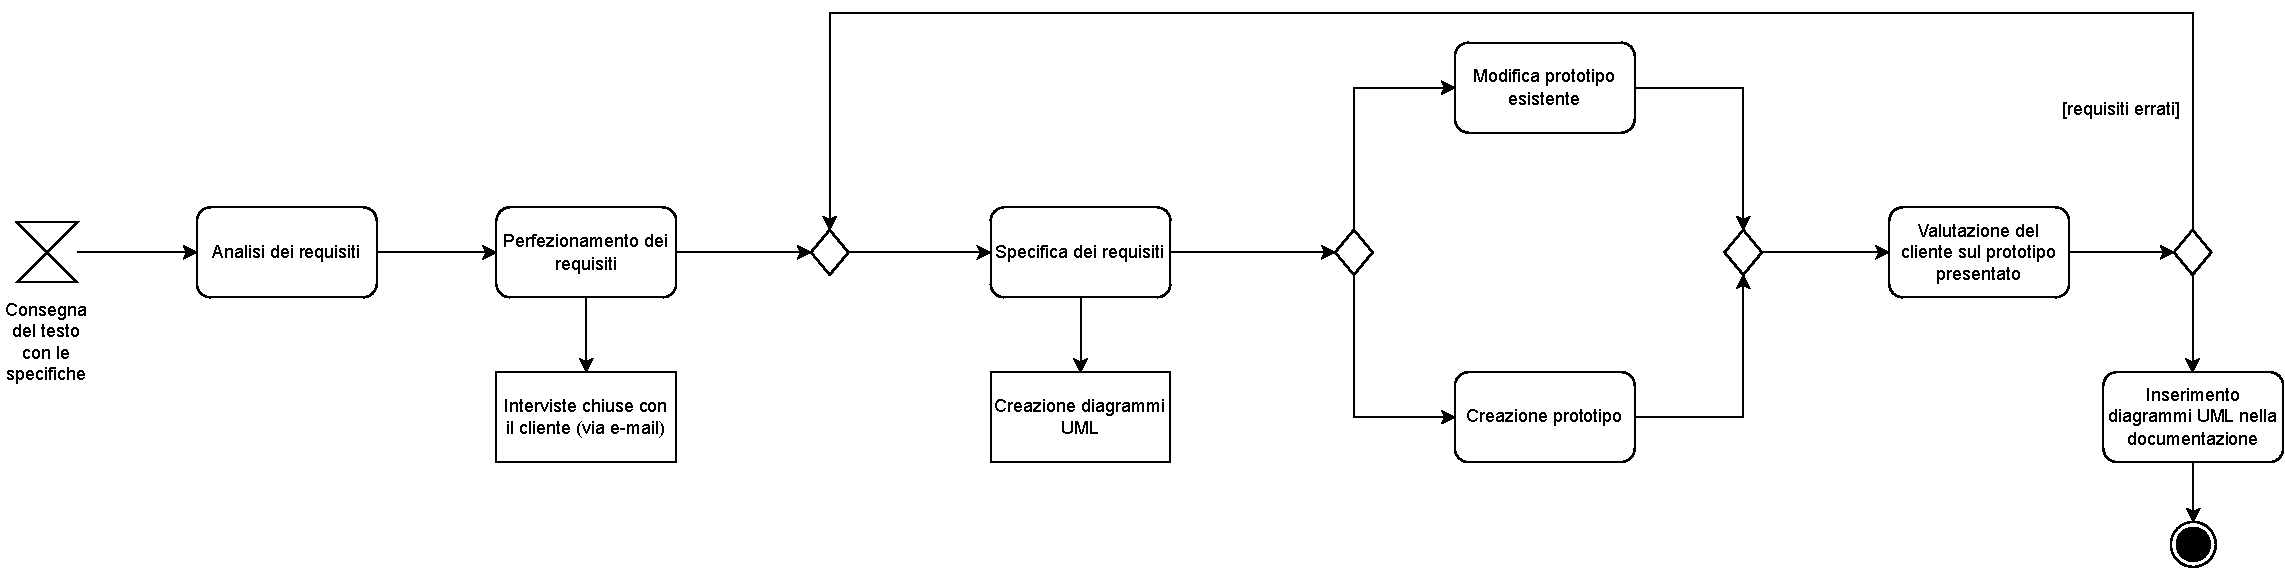
\includegraphics[width=1\textwidth]{diagrams/Activity_Diagram_-_Processo_ingegneria_dei_requisiti.pdf}
	\caption{Activity diagram - Processo di ingegneria dei requisiti}
	\label{fig:activity_diagram_-_Processo_ingegneria_dei_requisiti}
\end{figure}

\newpage


%%%%%%%%%%%%%%%%%%%%%%%%%%%%%%%%%%%%%%%%%%%%%%%%
%%%%%%%%%%%%% ANALISI DEI REQUISITI %%%%%%%%%%%%
%%%%%%%%%%%%%%%%%%%%%%%%%%%%%%%%%%%%%%%%%%%%%%%%
\subsection{Analisi dei requisiti}
Si vuole progettare un sistema informatico di una agenzia che fornisce servizi di supporto alla ricerca di lavoro stagionale. I lavoratori interessati possono iscriversi al servizio, rivolgendosi agli sportelli dell'agenzia. Il sistema deve permettere la gestione delle anagrafiche e la ricerca di lavoratori stagionali, nei settori dell'agricoltura e del turismo.
I responsabili, dipendenti dell'agenzia, devono inserire i dati dei lavoratori ed in particolare:
\begin{itemize}
	\item[\ding{213}] Dati anagrafici: nome, cognome, luogo e data di nascita, nazionalità;
	\item[\ding{213}] Indirizzo;
	\item[\ding{213}] [opzionale] Recapito telefonico personale;
	\item[\ding{213}] E-mail;
	\item[\ding{213}][opzionale] Specializzazioni/esperienze precedenti (bagnino, barman, istruttore di nuoto, viticultore, floricultore);
	\item[\ding{213}] Lingue parlate;
	\item[\ding{213}] Tipo di patente di guida;
	\item[\ding{213}] Se automunito;
	\item[\ding{213}] Periodi e zone (comuni), per il quale il lavoratore è disponibile;
	\item[\ding{213}] Almeno un contatto d'emergenza:
	\begin{enumerate}
		\item Nome;
		\item Cognome;
		\item E-mail;
		\item Telefono (opzionale);
	\end{enumerate}
	\item[\ding{213}] [opzionale] Lavori stagionali svolti negli ultimi 5 anni.
\end{itemize}
I dipendenti devono autenticarsi per poter accedere al sistema e inserire i dati dei lavoratori. Per ogni lavoro svolto vanno registrati:
\begin{itemize}
	\item[\ding{219}] Periodo;
	\item[\ding{219}] Nome dell'azienda;
	\item[\ding{219}] Mansioni svolte;
	\item[\ding{219}] Luogo di lavoro;
	\item[\ding{219}] Retribuzione lorda giornaliera;
\end{itemize}
Invece, per i dipendenti dell'agenzia si memorizzano:
\begin{itemize}
	\item[\ding{223}] Dati anagrafici;
	\item[\ding{223}] E-mail;
	\item[\ding{223}] Telefono;
	\item[\ding{223}] Credenziali di accesso (login e password);
\end{itemize}
Una volta registrate le informazioni sui lavoratori, il personale dell'agenzia può effettuare ricerche rispetto a possibili profili richiesti. In particolare, il sistema deve permettere ai dipendenti di effettuare ricerche per:
\begin{itemize}
	\item[\ding{112}] Lavoratore;
	\item[\ding{112}] Lingue parlate;
	\item[\ding{112}] Periodo di disponibilità;
	\item[\ding{112}] Mansioni indicate;
	\item[\ding{112}] Luogo di residenza;
	\item[\ding{112}] Disponibilità di auto/patente di guida;
\end{itemize}
Il sistema deve permettere di effettuare ricerche complesse, attraverso la specifica di differenti condizioni di ricerca (sia in AND che in OR).

\newpage


%%%%%%%%%%%%%%%%%%%%%%%%%%%%%%%%%%%%%%%%%%%%%%%%
%%%%%%%% PERFEZIONAMENTO DEI REQUISITI %%%%%%%%%
%%%%%%%%%%%%%%%%%%%%%%%%%%%%%%%%%%%%%%%%%%%%%%%%
\subsection{Perfezionamento dei requisiti}
L'intervista con il cliente è stata eseguita tramite uno scambio di messaggi via e-mail.\\
Qui di seguito si lascia un elenco con domanda e risposta:
\begin{itemize}
	\item[\ding{45}] Quando vengono definiti i dati da memorizzare per ogni lavoratore, viene menzionato luogo di nascita. Invece, quando vengono elencati i parametri di ricerca, viene richiesto il luogo di residenza. Se quest'ultimo non viene inserito, come è possibile ricavarlo?
	\begin{itemize}
		\item[\ding{42}] L’indirizzo del lavoratore è ovviamente corrispondente al luogo di residenza.
	\end{itemize}

	\item[\ding{45}] Il sistema non richiede esplicitamente un portale per la gestione dei responsabili, ovvero l'inserimento dei loro dati e le relative credenziali. Provvederà il team di sviluppo a implementare tale funzione in modo dettagliato o sarà lasciato come opzione ad ogni dipendente?
	\begin{itemize}
		\item[\ding{42}] Un responsabile \textbf{non} deve poter avere accesso ad una eventuale gestione dei dipendenti. Tuttavia, la decisione su come gestire, inserire, modificare e/o eliminare un responsabile, non è ben chiara al cliente.\\
		Quindi, si lascia carta bianca al team di sviluppo.
	\end{itemize}
	
	\item[\ding{45}] Le eventuali esperienze/specializzazioni richieste sono indicate tra parentesi. L'agenzia è interessate solo a queste o anche ad altre?
	\begin{itemize}
		\item[\ding{42}] Le specializzazioni, o esperienze passate, sono quelle indicate tra parentesi. Il target a cui è rivolto questo software non ha interesse ad essere a conoscenza di altro.
	\end{itemize}

	\item[\ding{45}] La gestione delle anagrafiche deve consentire la modifica di \textbf{tutti} i dati inseriti o solo alcuni?
	\begin{itemize}
		\item[\ding{42}] Tutti i dati inseriti. È possibile che nel momento dell'inserimento un responsabile faccia un errore di battitura, oppure che il lavoratore cambi eventuali dati (nome, indirizzo, telefono, ecc.). Il sistema deve quindi consentire di avere il pieno controllo.
	\end{itemize}
\end{itemize}

\newpage


%%%%%%%%%%%%%%%%%%%%%%%%%%%%%%%%%%%%%%%%%%%%%%%%
%%%%%%%%%%% SPECIFICA DEI REQUISITI %%%%%%%%%%%%
%%%%%%%%%%%%%%%%%%%%%%%%%%%%%%%%%%%%%%%%%%%%%%%%
\subsection{Specifica dei requisiti}
\subsubsection{Casi d'uso generali}
Si presenta un unico diagramma raffigurante i casi d'uso esistenti. Il sistema si pone l'obbiettivo di supportare l'azienda fornendo servizi per la ricerca di lavoro stagionale.\\
Il sistema ha come protagonista due attori: il ``responsabile'' e ``admin''. Il primo, come dice la parola stessa, è il responsabile che ha il compito di registrare eventuali lavoratori, di effettuare modifiche o ricerche. Il secondo, invece, è l'amministratore (\emph{admin}) che gestisce i vari responsabili modificando, eliminando o inserendone di nuovi.
% Use case
\begin{figure}[htpb]
	\centering
	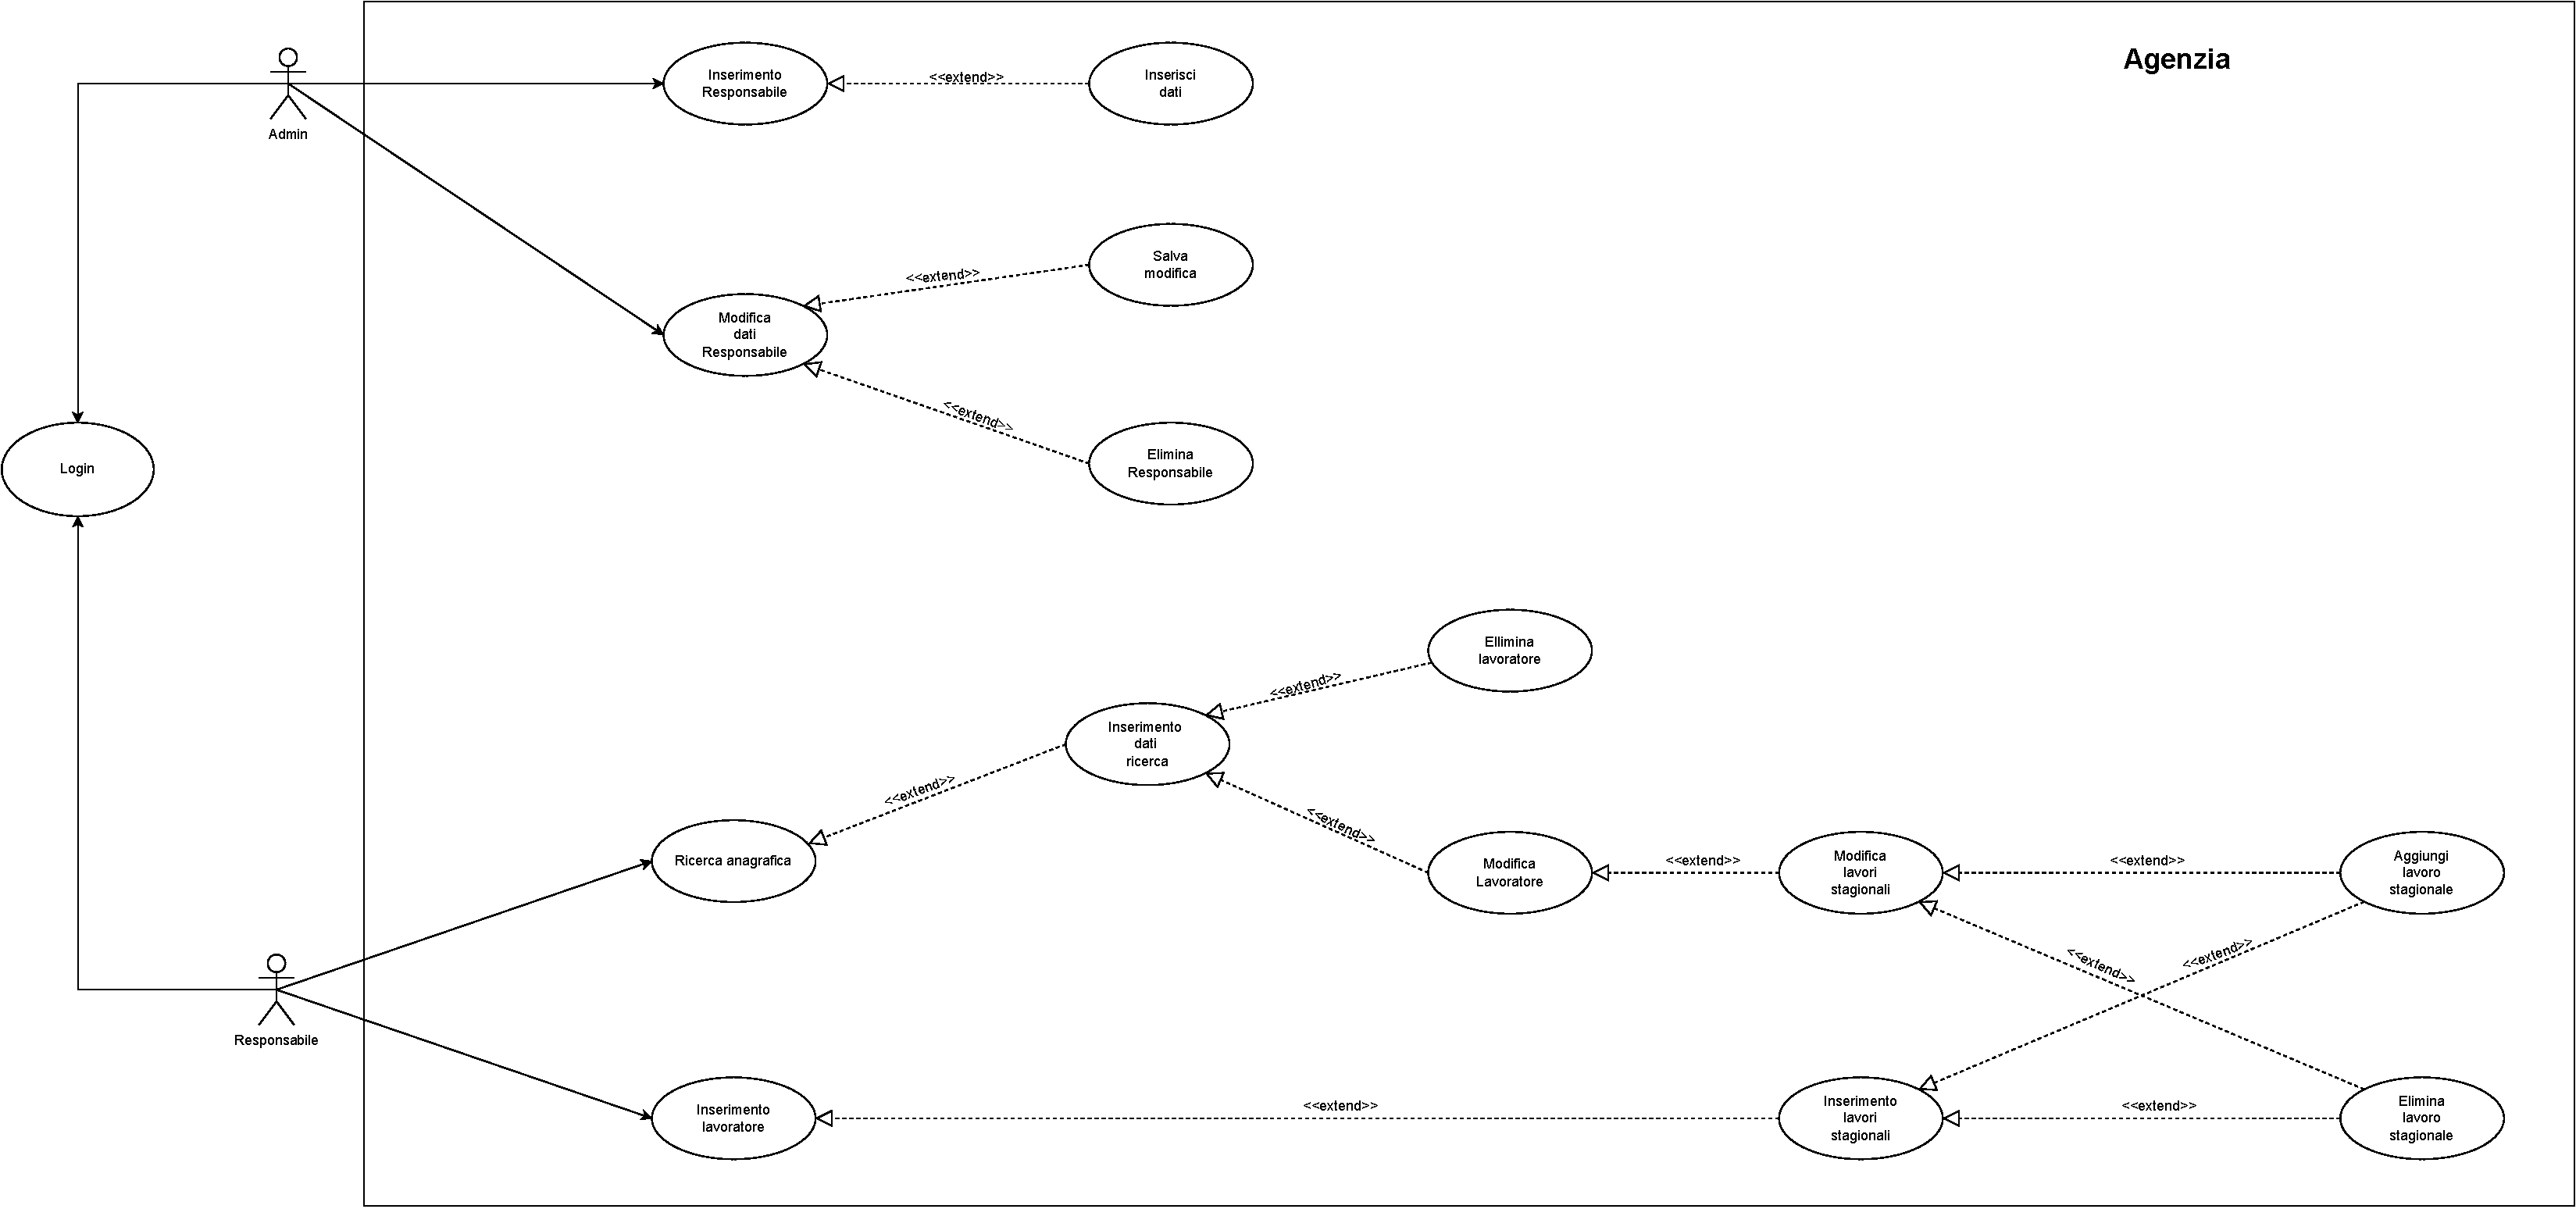
\includegraphics[width=1\textwidth]{diagrams/Use_case.pdf}
	\caption{Use case}
	\label{fig:use_case}
\end{figure}

\newpage
\begin{center}
	\title{\textbf{Accesso al sistema - Login}}
	\maketitle
\end{center}
Sia il responsabile che admin, per poter accedere al sistema, devono inserire le loro credenziali. Una volta inserite, viene premuto LOGIN per eseguire l'accesso. Se sono corrette, l'utente accede al sistema, altrimenti dovrà riprovare.\\
\:\\
Dato che il login è identico sia per il responsabile che per admin, il caso d'uso e il relativo diagramma di flusso vengono rappresentati in modo generale.
\begin{center}	
	\begin{tabular}{|c|}
		\hline
		\textbf{Use case: Login}\\
		\hline	
		\textbf{Attori:} Utente\\
		\hline
		\textbf{Precondizioni:}\\Inserimento delle credenziali\\
		\hline
		\textbf{Sequenza degli eventi:}\\
		\begin{minipage}{5in}
			\begin{enumerate}
				\item L'utente clicca "Login"
				\item Se le credenziali sono corrette:
				\begin{enumerate}
					\item Viene dato l'accesso alla interfaccia successiva
				\end{enumerate}
				\item Altrimenti viene restituito un errore\\
			\end{enumerate}
		\end{minipage}\\
		\hline
		\textbf{Sequenza alternativa:}\\
		\begin{minipage}{5in}
			\begin{enumerate}
				\item L'utente può in qualsiasi momento terminare il programma\\
			\end{enumerate}
		\end{minipage}\\
		\hline
		\textbf{Postcondizioni:}\\
		\begin{minipage}{5in}
			\begin{enumerate}
				\item Verrà generata una nuova interfaccia in base al tipo di credenziali: amministrative o responsabile\\
			\end{enumerate}
		\end{minipage}\\
		\hline
	\end{tabular}
\end{center}
% Sequence_Diagram_-_Login_1
\begin{figure}[htpb]
	\centering
	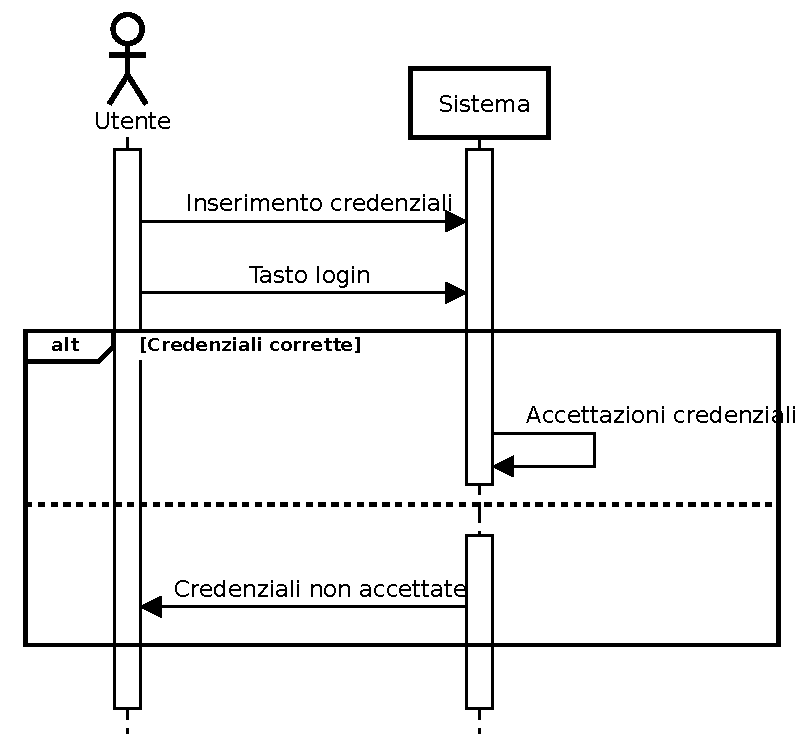
\includegraphics[width=1\textwidth]{diagrams/Sequence_Diagram_-_Login_1.pdf}
	\caption{Sequence Diagram - Login}
	\label{fig:seq_dia_login}
\end{figure}




\newpage

\subsubsection{Casi d'uso admin}
\begin{center}
	\title{\textbf{Inserimento responsabile}}
	\maketitle
\end{center}
L'unico attore per questo caso d'uso è admin.\\
\:\\
Il sistema fornisce la possibilità di:
\begin{itemize}
	\item[\ding{51}] Visualizzare l'intero elenco di responsabili presenti nel sistema;
	\item[\ding{51}] Inserire nuovi responsabili;
	\item[\ding{51}] Modificare i responsabili;
	\item[\ding{51}] Eliminare i responsabili.
\end{itemize}
Quindi, il software garantisce un controllo \underline{totale} dei responsabili.\\
Inoltre, per motivi di privacy, le password preesistenti non possono essere visualizzate da admin, ma solamente sovrascritte con una nuova.
\begin{center}
	\begin{tabular}{|c|}
		\hline
		\textbf{Use case: Inserimento responsabile}\\
		\hline	
		\textbf{Attori:} Admin\\
		\hline
		\textbf{Precondizioni:}\\ Login effettuato con successo utilizzando le credenziali amministrative\\
		\hline
		\textbf{Sequenza degli eventi:}\\
		\begin{minipage}{5in}
			\begin{enumerate}
				\item L'amministratore inserisce i dati del nuovo responsabile
				\item Fintantochè l'amministratore è nella pagina di inserimento, Se preme il tasto "salva":
				\begin{enumerate}
					\item Le modifiche vengono salvate permanentemente 
				\end{enumerate}
				\item Se preme il pulsante "indietro":
				\begin{enumerate}
					\item Ritorna alla pagina iniziale di login
				\end{enumerate}
				\item Se preme il tasto "modifica"
				\begin{enumerate}
					\item I campi vengono autocompilati con quelli del responsabile
					\item L'amministratore li modifica in accordo alle sue specifiche
				\end{enumerate}
				\item Se il responsabile clicca il pulsante "elimina":
				\begin{enumerate}
					\item Il responsabile viene eliminato dalla lista\\
				\end{enumerate}
			\end{enumerate}
		\end{minipage}\\
		\hline
		\textbf{Sequenza alternativa:}\\
		\begin{minipage}{5in}
			\begin{enumerate}
				\item L'amministratore clicca il pulsante indietro e torna alla pagina di login scartando ogni modifica effettuata o terminare il programma\\
			\end{enumerate}
		\end{minipage}\\
		\hline
	\end{tabular}
\end{center}
% Sequence_Diagram_-_InsResp_1
\begin{figure}[htpb]
	\centering
	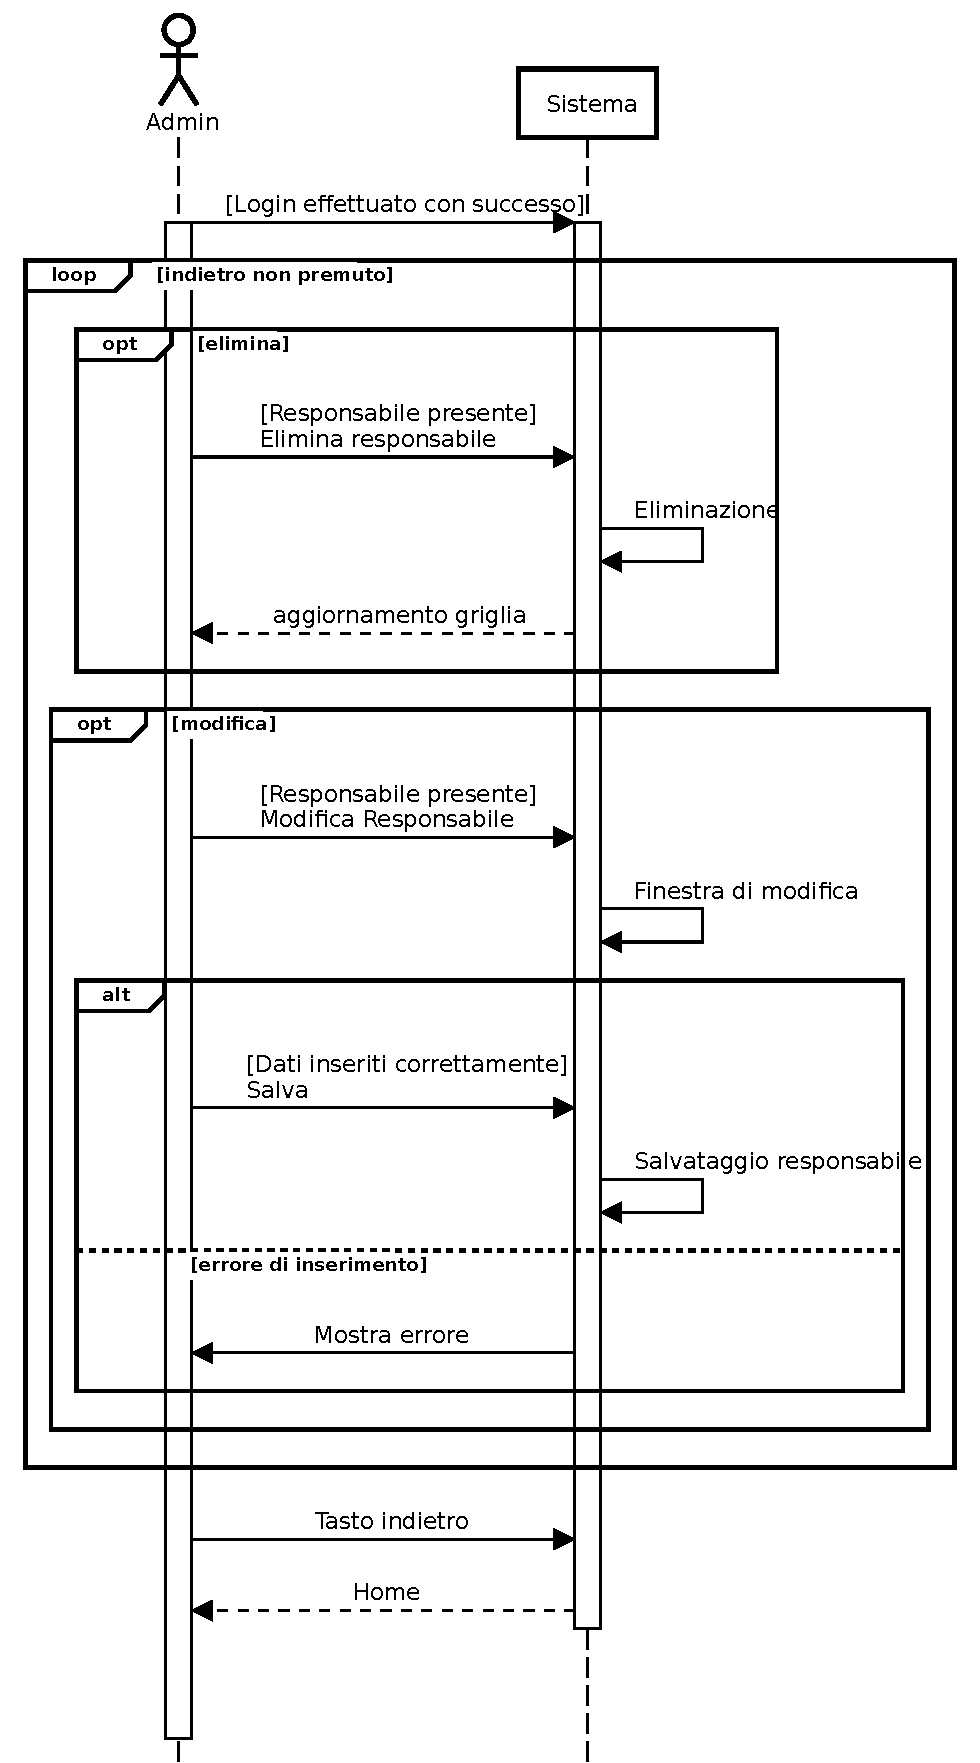
\includegraphics[width=0.9\textwidth]{diagrams/Sequence_Diagram_-_InsResp_1.pdf}
	\caption{Sequence Diagram - Inserimento responsabile}
	\label{fig:seq_dia_ins_resp}
\end{figure}




\newpage

\subsubsection{Casi d'uso responsabile}
\begin{center}
	\title{\textbf{Inserimento lavoratore}}
	\maketitle
\end{center}
Una volta effettuato il login e selezionato l'inserimento del lavoratore, il responsabile ha la possibilità di inserire tutti i dati di un lavoratore.\\
In questa schermata viene data la possibilità di inserire tutti i dati del lavoratore \underline{eccetto} i lavori stagionali.\\
Infine, esiste la possibilità, in qualsiasi momento, di tornare alla schermata precedente grazie al pulsante INDIETRO.\\\:\\
\underline{\textbf{NOTA}}: il sequence diagram è stato creato in unione con il caso d'uso ``Inserimento lavoro stagionale'' (prossima pagina).
\begin{center}
	\begin{tabular}{|c|}
		\hline
		\textbf{Use case: Inserimento lavoratore}\\
		\hline	
		\textbf{Attori:} Responsabile\\
		\hline
		\textbf{Precondizioni:}\\ Login effettuato con successo\\
		\hline
		\textbf{Sequenza degli eventi:}\\
		\begin{minipage}{5in}
			\begin{enumerate}
				\item Il responsabile clicca "Inserimento dati lavoratori":
				\item Inserisce i dati del lavoratore da aggiungere alla anagrafica
				\item Clicca "avanti" e procede alla pagina di aggiunta dei lavori stagionali\\
			\end{enumerate}
		\end{minipage}\\
		\hline
		\textbf{Sequenza alternativa:}\\
		\begin{minipage}{5in}
			\begin{enumerate}
				\item Il responsabile può in qualsiasi momento tornare indietro alla pagina home o terminare il programma\\
			\end{enumerate}
		\end{minipage}\\
		\hline
		\textbf{Postcondizioni:}\\
		\begin{minipage}{5in}
			\begin{enumerate}
				\item Il lavoratore viene salvato temporaneamente senza alcun lavoro stagionale inserito\\
			\end{enumerate}
		\end{minipage}\\
		\hline
	\end{tabular}
\end{center}

\newpage
\begin{center}
	\title{\textbf{Inserimento lavoro stagionale}}
	\maketitle
\end{center}
Questa schermata consente di inserire molteplici lavori stagionali.\\
Il responsabile ha dunque la possibilità di aggiungere un lavoro stagionale ed eventualmente eliminarlo nel caso in cui abbia commesso errori durante l'inserimento.\\
Il sistema, dopo che il responsabile ha cliccato sul tasto AGGIUNGI, inserisce il lavoro stagionale nell'apposita tabella.\\
Il software è flessibile, dunque non costringe l'utente ad inserire obbligatoriamente almeno un lavoro stagionale, ma lascia la libertà di salvare, tramite il tasto FINE, in qualsiasi momento.\\
Infine il sistema consente di tornare indietro, mantenendo i dati in precedenza inseriti, alla pagina di inserimento.
\begin{center}
	\begin{tabular}{|c|}
		\hline
		\textbf{Use case: Inserimento lavoro stagionale}\\
		\hline	
		\textbf{Attori:} Responsabile\\
		\hline
		\textbf{Precondizioni:}\\ Login effettuato con successo\\
		\hline
		\textbf{Sequenza degli eventi:}\\
		\begin{minipage}{5in}
			\begin{enumerate}
				\item Il responsabile compila i campi preposti con i dati relativi al lavoro stagionale
				\item Preme il tasto "aggiungi" ed esegue la aggiunta del lavoro effettuato
				\item Fintantochè resta nella pagina di inserimento, Se preme il tasto "fine":
				\begin{enumerate}
					\item Rende permanente la aggiunta del lavoratore e dei lavori stagionali
					\item Torna alla pagina home con la scelta della operazione che può effettuare
				\end{enumerate}
				\item Se preme il tasto "elimina" accanto a un lavoro stagionale:
				\begin{enumerate}
					\item Elimina il lavoro stagionale inserito\\
				\end{enumerate}	
			\end{enumerate}
		\end{minipage}\\
		\hline
		\textbf{Sequenza alternativa:}\\
		\begin{minipage}{5in}
			\begin{enumerate}
				\item Il responsabile può in qualsiasi momento tornare indietro alla pagina home o terminare il programma\\
			\end{enumerate}
		\end{minipage}\\
		\hline
	\end{tabular}
\end{center}
% Sequence_Diagram_-_Inserimento-lavoratore_1
\begin{figure}[htpb]
	\centering
	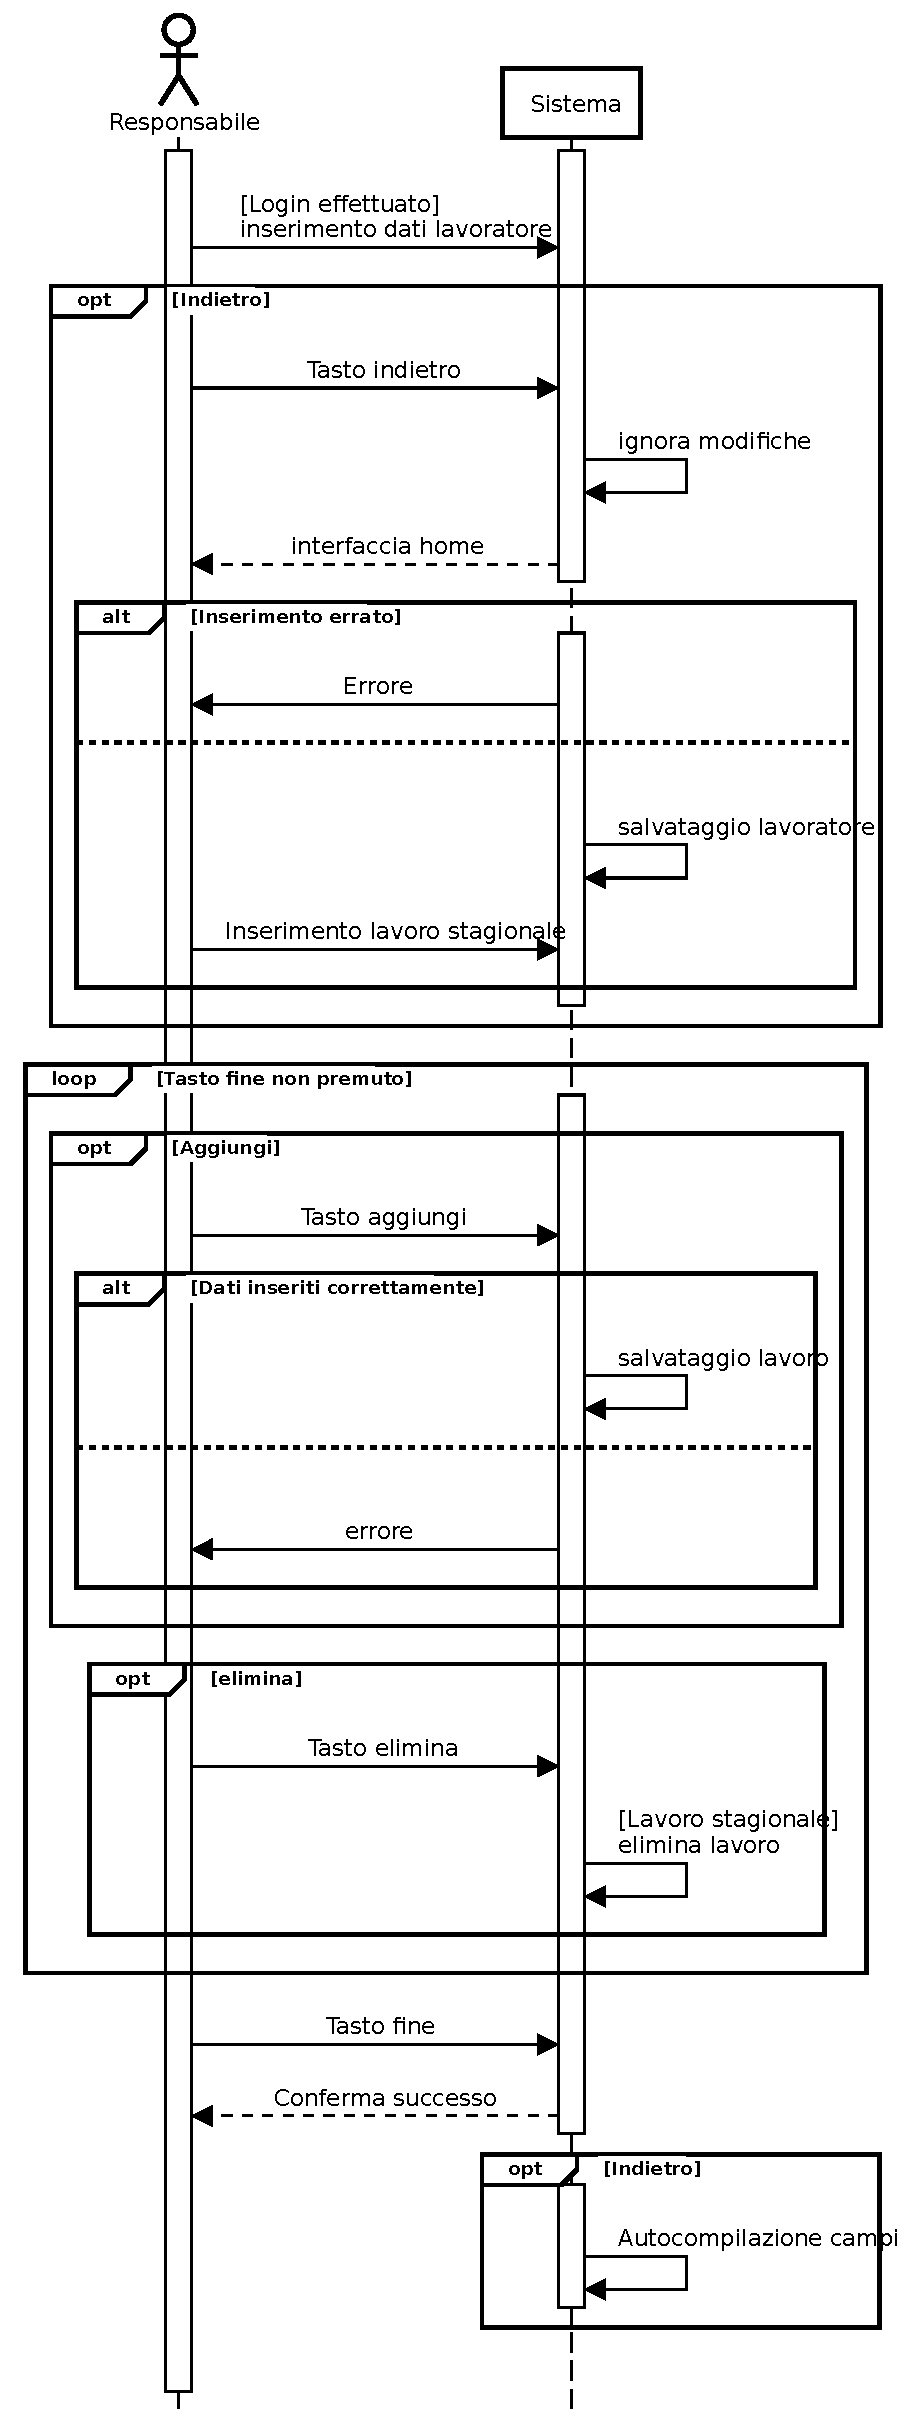
\includegraphics[width=0.6\textwidth]{diagrams/Sequence_Diagram_-_Inserimento-lavoratore_1.pdf}
	\caption{Sequence Diagram - Inserimento lavoratore e lavoro stagionale}
	\label{fig:seq_dia_ins_lavoratore}
\end{figure}

\newpage
\begin{center}
	\title{\textbf{Ricerca anagrafica}}
	\maketitle
\end{center}
Questa schermata consente di eseguire una ricerca dei lavoratori all'interno di tutto il sistema.\\
Il software è flessibile e consente al responsabile di effettuare ricerche molto avanzate utilizzando operatori logici: AND e OR. Inoltre, ogni campo può essere combinato con altri tramite questi due operatori per creare ricerche ancora più dettagliate.\\
Il sistema consente anche di modificare ed eliminare i lavoratori.
\begin{center}
	\begin{tabular}{|c|}
		\hline
		\textbf{Use case: Ricerca anagrafica}\\
		\hline	
		\textbf{Attori:} Responsabile\\
		\hline
		\textbf{Precondizioni:}\\ Login effettuato con successo\\
		\hline
		\textbf{Sequenza degli eventi:}\\
		\begin{minipage}{5in}
			\begin{enumerate}
				\item Il responsabile clicca "Ricerca e aggiornamento anagrafiche"
				\item Fintantochè resta nella pagina di aggiornamento e ricerca, Se preme il tasto "mostra tutti"
				\begin{enumerate}
					\item Visualizza tutti i lavoratori attualmente presenti nella anagrafica
				\end{enumerate}
				\item Se preme il tasto "cerca":
				\begin{enumerate}
					\item Mostra i risultati della ricerca effettuata in base ai campi compilati
				\end{enumerate}
				\item Se preme il tasto "modifica" a fianco di un lavoratore:
				\begin{enumerate}
					\item Verrà rimandato alla pagina di inserimento del lavoratore con i campi precompilati per procedere alla modifica
				\end{enumerate}
				\item Se preme il tasto "elimina":
				\begin{enumerate}
					\item Il lavoratore con i relativi dati e i lavori stagionali eventualmente inseriti verrà eliminato definitivamente\\
				\end{enumerate}
			\end{enumerate}
		\end{minipage}\\
		\hline
		\textbf{Sequenza alternativa:}\\
		\begin{minipage}{5in}
			\begin{enumerate}
				\item Il responsabile può in qualsiasi momento tornare indietro alla pagina home o terminare il programma\\
			\end{enumerate}
		\end{minipage}\\
		\hline
	\end{tabular}
\end{center}
% Sequence_Diagram_-_Ricerca-anagrafica_1
\begin{figure}[htpb]
	\centering
	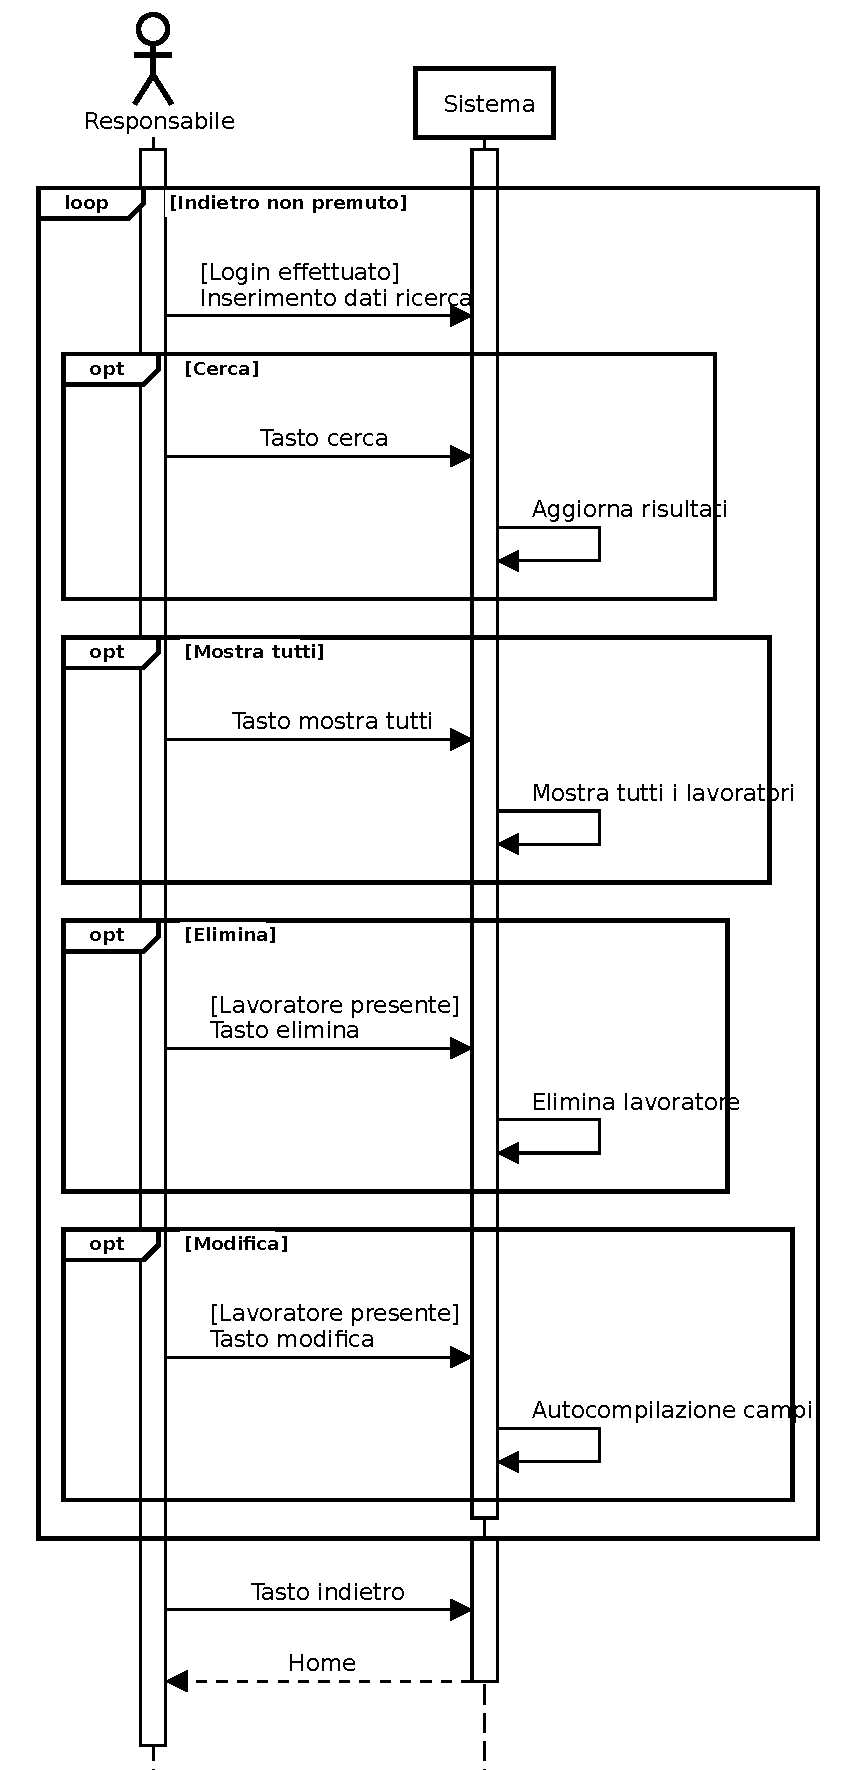
\includegraphics[width=0.76\textwidth]{diagrams/Sequence_Diagram_-_Ricerca-anagrafica_1.pdf}
	\caption{Sequence Diagram - Ricerca anagrafica}
	\label{fig:seq_dia_ric_anagrafica}
\end{figure}




\newpage

\subsubsection{Diagramma di attività}
\underline{\textbf{NOTA}}: I seguenti diagrammi hanno l'obbiettivo di essere completi e chiari al lettore. Tuttavia, non è stato possibile inserire casi particolari, come la chiusura del software, o l'esecuzione di molteplici operazioni in sequenza casuale. Sono stati previsti i casi in cui si ripeta l'operazione più di una volta, ma si tratta comunque di situazioni semplici.\\
Queste scelte sono state effettuate per evitare di rendere difficile la lettura dei diagrammi.
\begin{center}
	\title{\textbf{Accesso al sistema - Login}}
	\maketitle
\end{center}
% Activity_Diagram_-_Login
\begin{figure}[htpb]
	\centering
	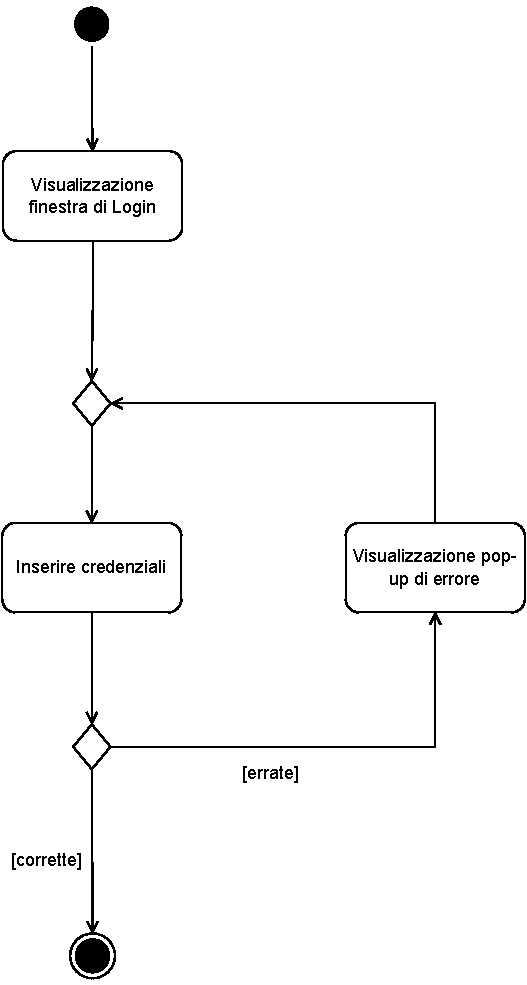
\includegraphics[width=0.61\textwidth]{diagrams/Activity_Diagram_-_Login.pdf}
	\caption{Activity Diagram - Accesso al sistema - Login}
	\label{fig:act_dia_login}
\end{figure}


\newpage


\begin{center}
	\title{\textbf{Attività del responsabile}}
	\maketitle
\end{center}
% Activity_Diagram_-_Responsabile
\begin{figure}[htpb]
	\centering
	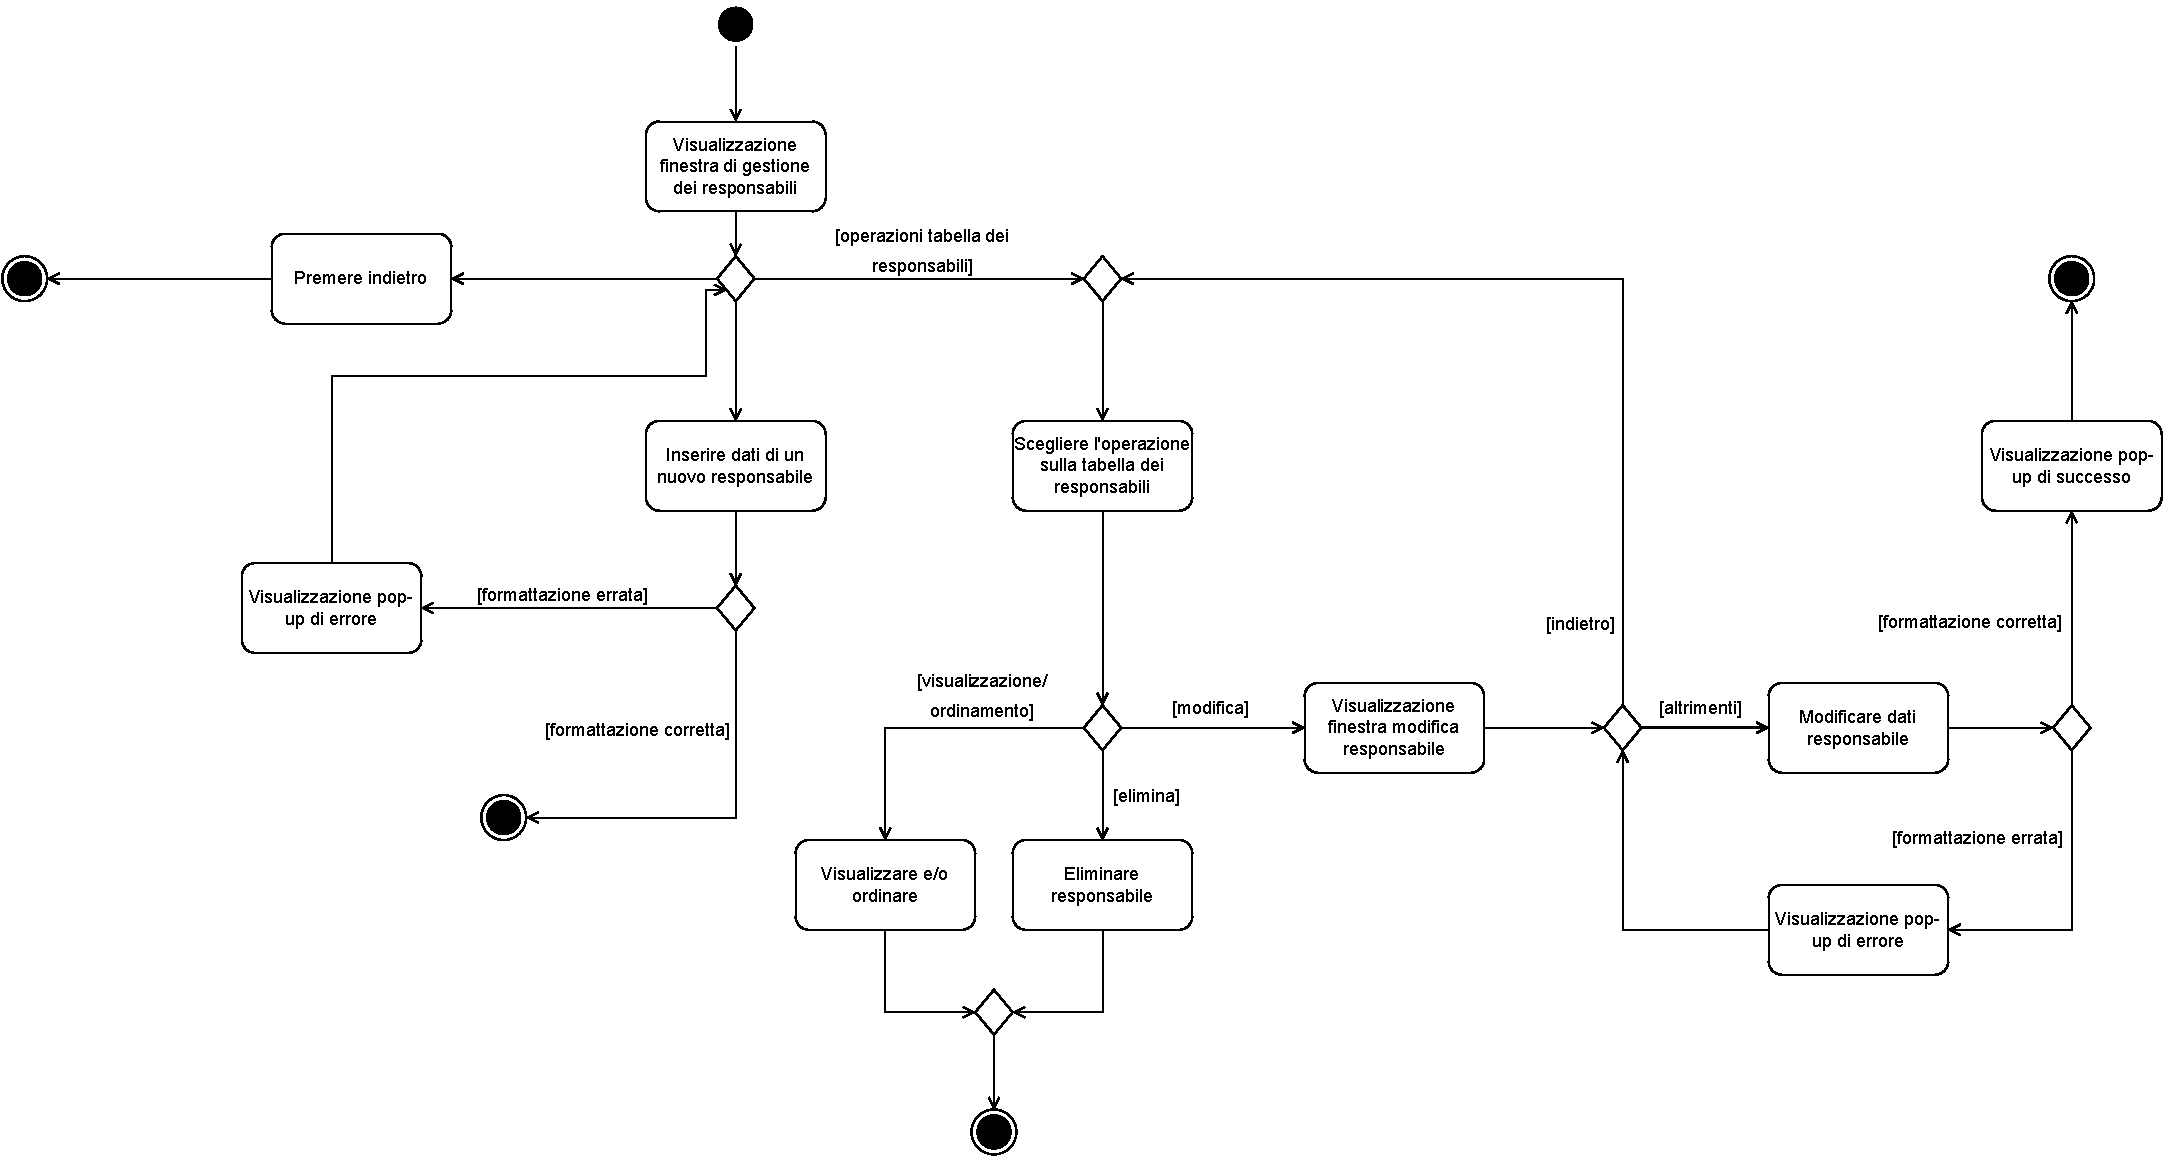
\includegraphics[width=1.2\textwidth]{diagrams/Activity_Diagram_-_Responsabile.pdf}
	\caption{Activity Diagram - Attività del responsabile}
	\label{fig:act_dia_resp}
\end{figure}


\newpage


\begin{center}
	\title{\textbf{Selezione dell'operazione da parte del responsabile}}
	\maketitle
\end{center}
% Activity_Diagram_-_Selezione
\begin{figure}[htpb]
	\centering
	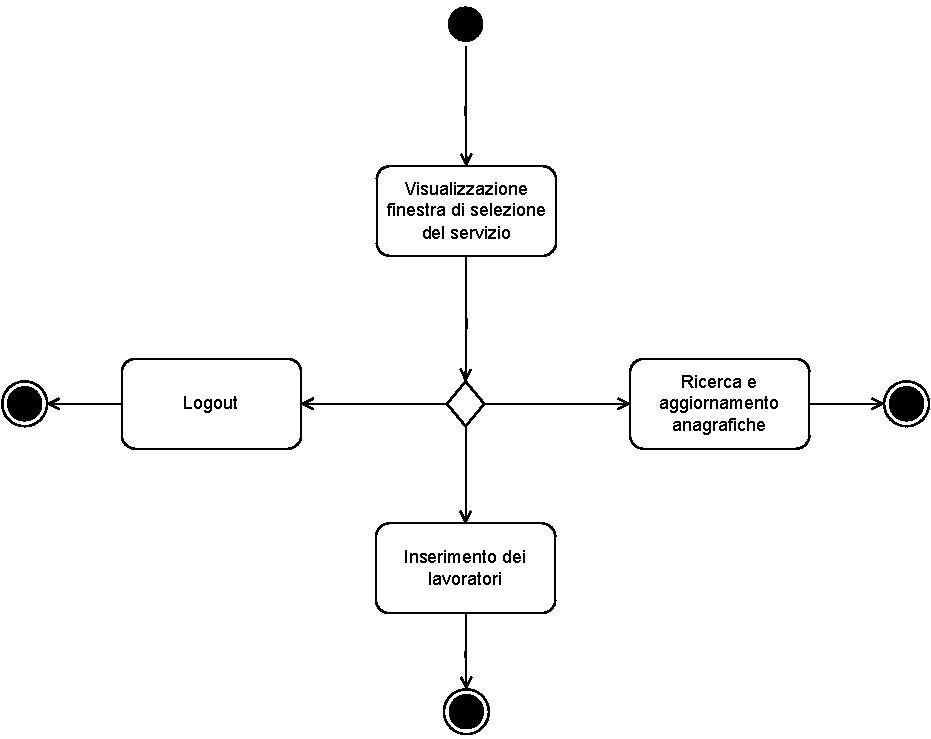
\includegraphics[width=1\textwidth]{diagrams/Activity_Diagram_-_Selezione.pdf}
	\caption{Activity Diagram - Selezione dell'operazione da parte del responsabile}
	\label{fig:act_dia_selezione}
\end{figure}


\newpage


\begin{center}
	\title{\textbf{Inserimento lavoratore da parte del responsabile}}
	\maketitle
\end{center}
% Activity_Diagram_-_Inserimento_dati_lavoratori
\begin{figure}[htpb]
	\centering
	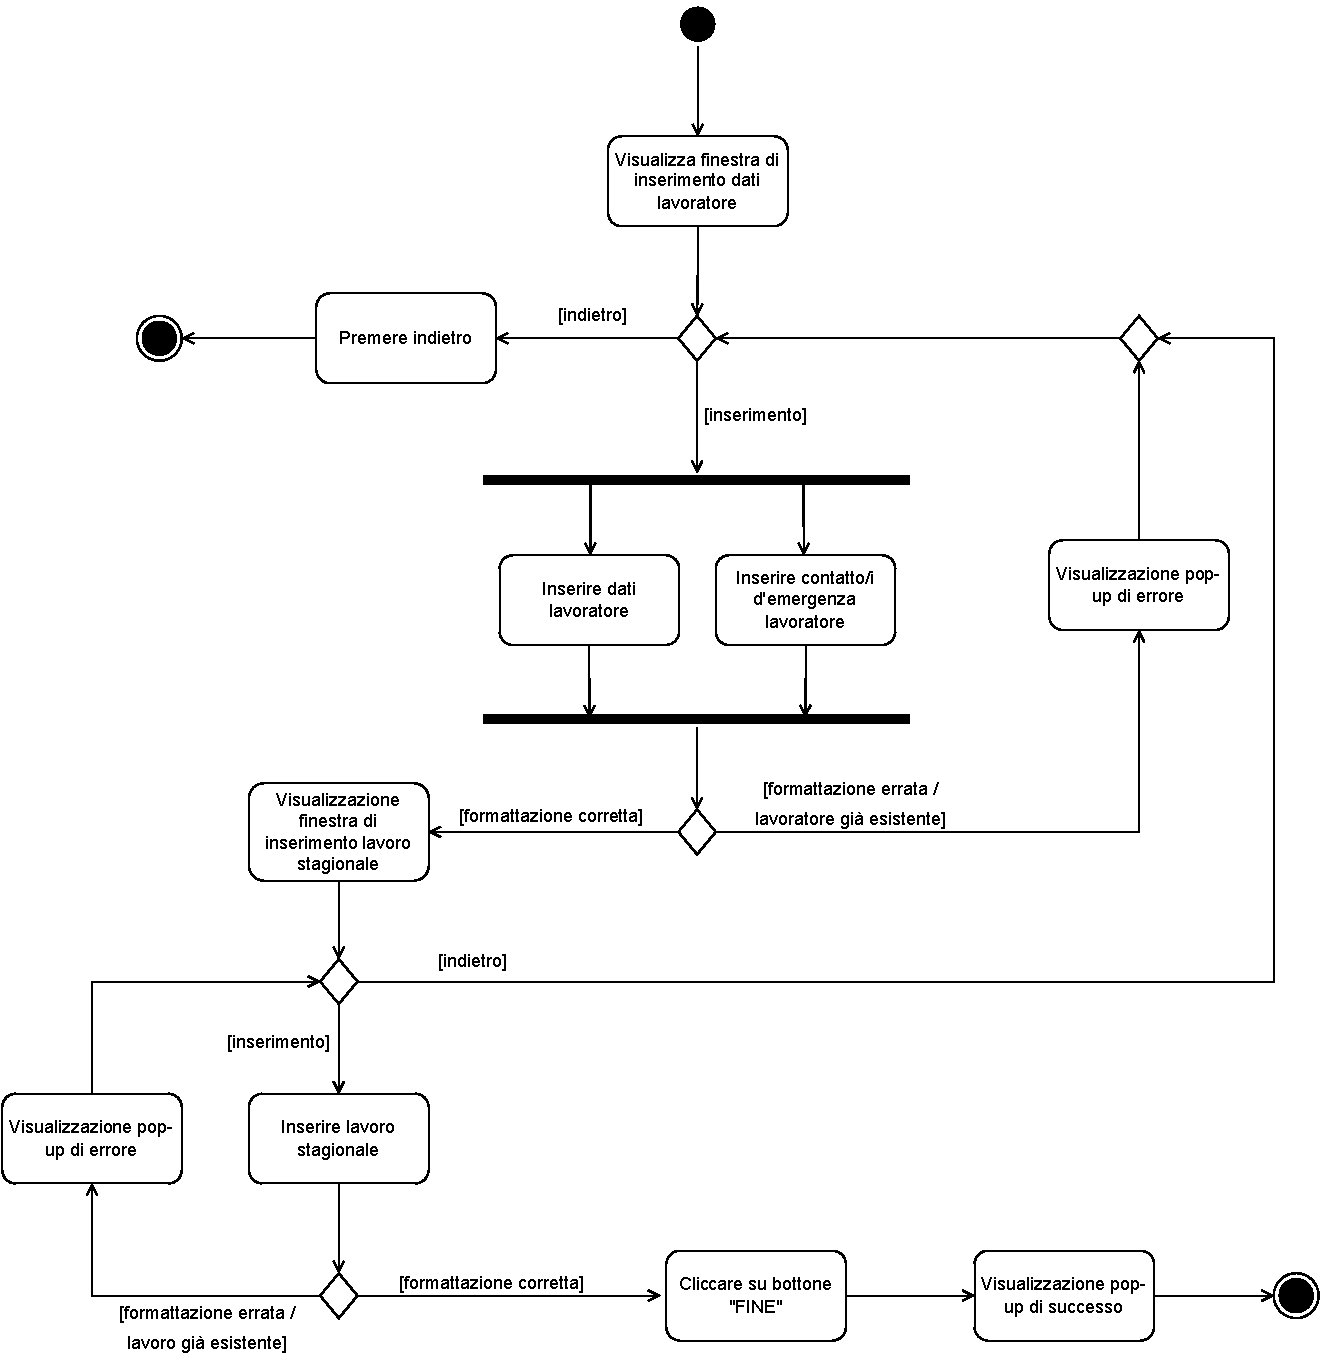
\includegraphics[width=1\textwidth]{diagrams/Activity_Diagram_-_Inserimento_dati_lavoratori.pdf}
	\caption{Activity Diagram - Inserimento lavoratore da parte del responsabile}
	\label{fig:act_dia_ins_lav}
\end{figure}


\newpage


\begin{center}
	\title{\textbf{Ricerca anagrafica da parte del responsabile}}
	\maketitle
\end{center}
% Activity_Diagram_-_Ricerca_anagrafiche
\begin{figure}[htpb]
	\centering
	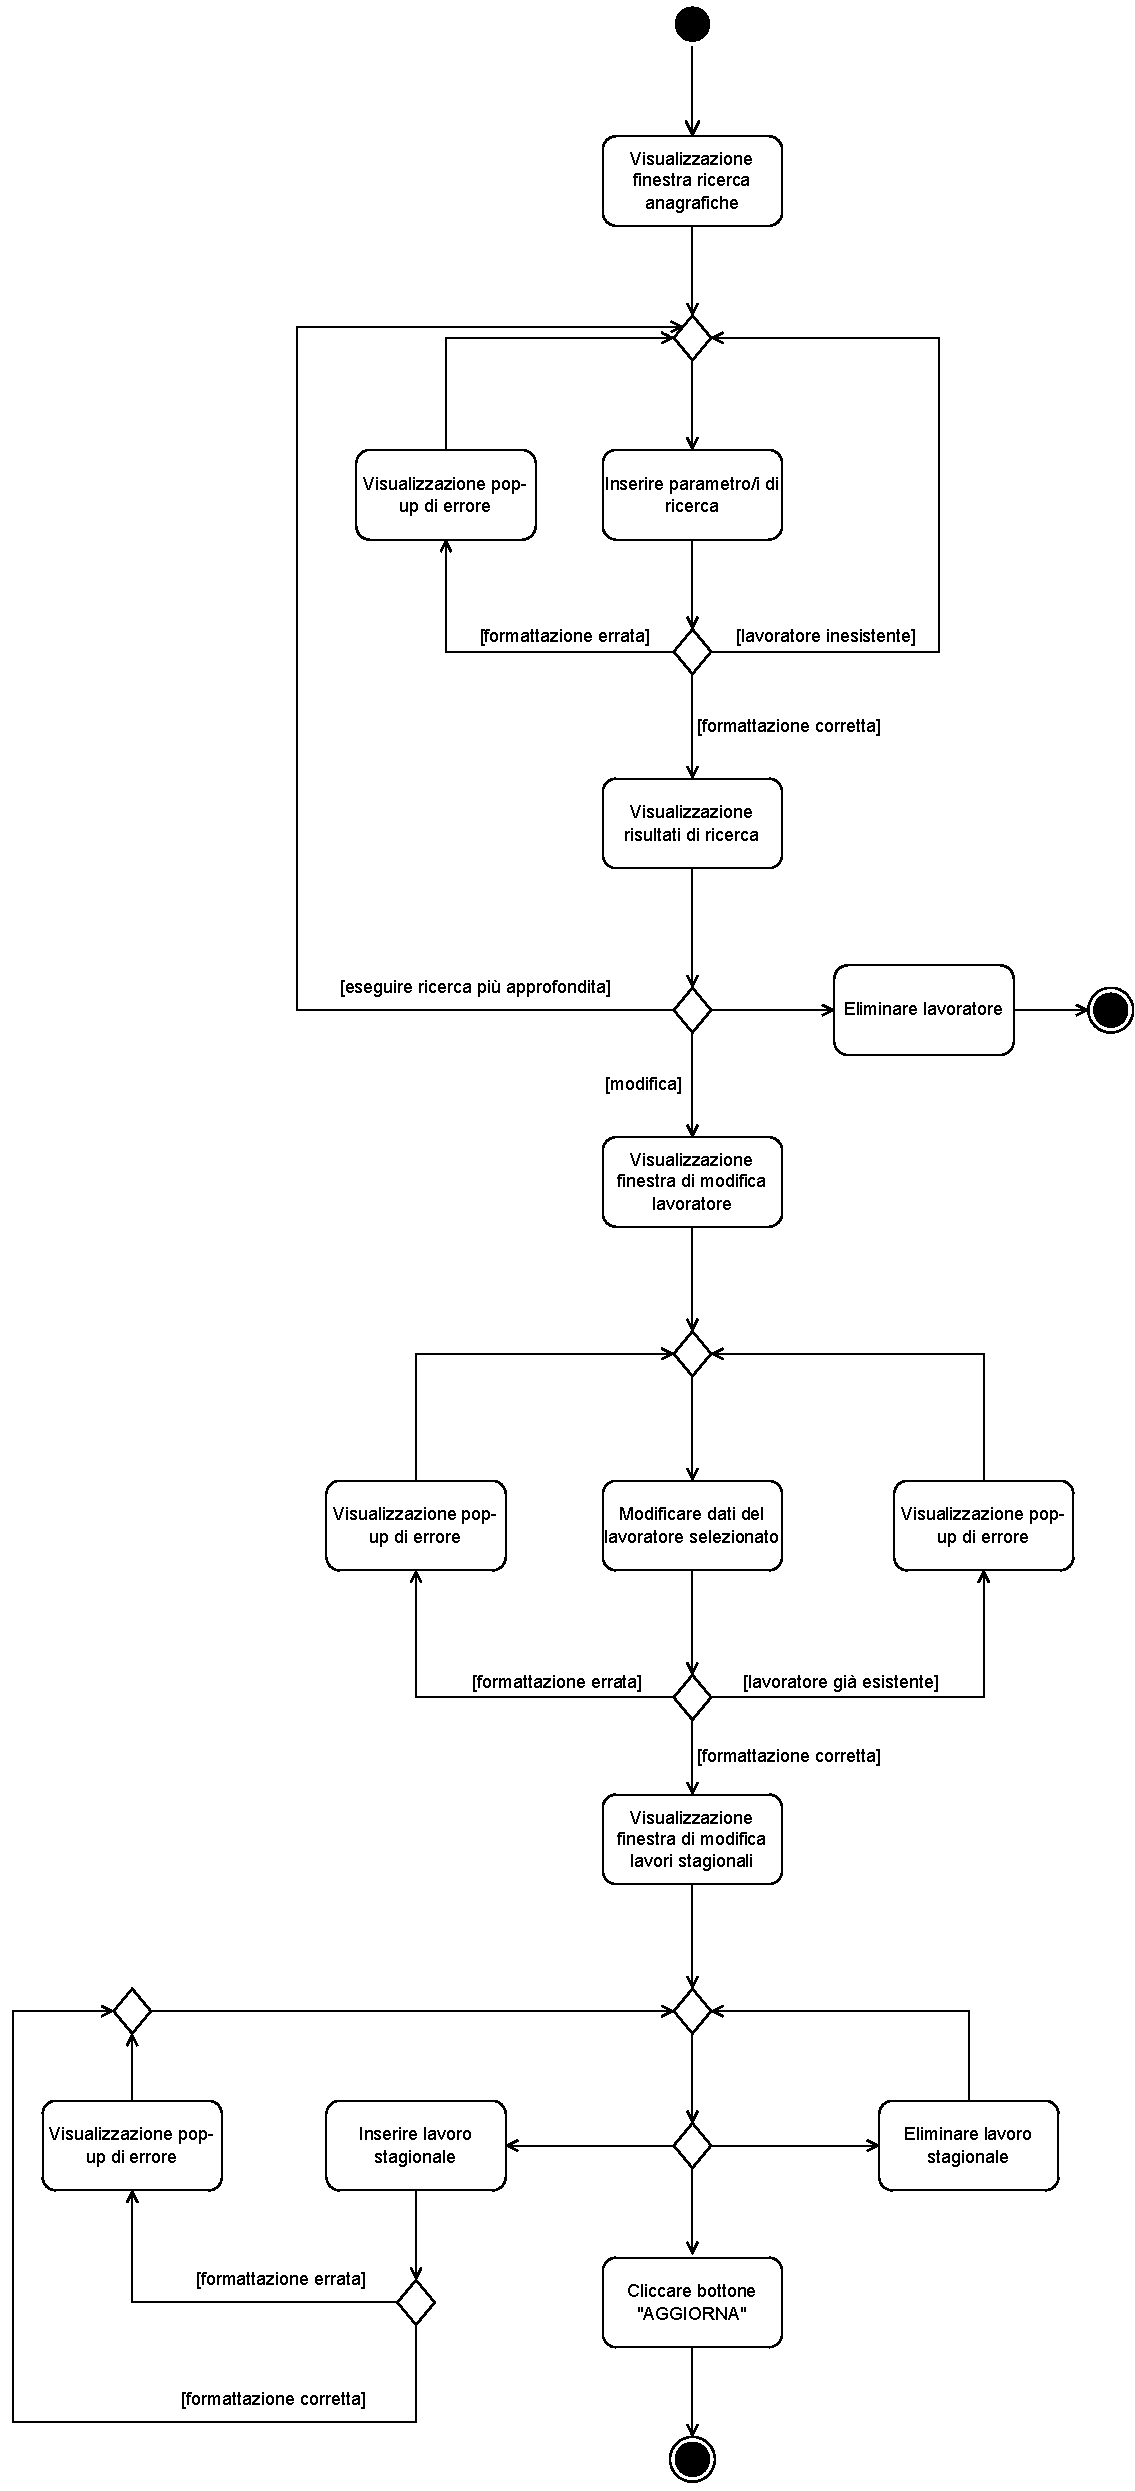
\includegraphics[width=0.55\textwidth]{diagrams/Activity_Diagram_-_Ricerca_anagrafiche.pdf}
	\caption{Activity Diagram - Ricerca anagrafica da parte del responsabile}
	\label{fig:act_dia_ric_ana}
\end{figure}


\newpage
%%%%%%%%%%%%%%%%%%%%%%%%%%%%%%%%%%%%%%%%%%%%%%%%
%%%%% IMPLEMENTAZIONE E SVILUPPO SOFTWARE %%%%%%
%%%%%%%%%%%%%%%%%%%%%%%%%%%%%%%%%%%%%%%%%%%%%%%%
\section{Implementazione e sviluppo software}
\label{sec:imp_svil}
\subsection{Processo di sviluppo}
Durante il processo di sviluppo è stato utilizzato il metodo \textbf{Agile ed Incrementale}.\\
Il metodo agile scelto è stato \textbf{Scrum}. Nonostante sia consigliato per aziende di medie/grandi dimensioni grazie alla sua chiara visibilità esterna, il team di sviluppo ha ottenuto ottimi risultati con l'applicazione di questo sistema.\\
\:\\
Il team di sviluppo è composto da tre persone e inizialmente è stato stilato un \textbf{\emph{product backlog}}, ovvero una lista di elementi di cui si deve occupare il team.\\
Una volta definiti i compiti, sono stati programmati degli \textbf{\emph{sprint}}, cioè dei periodi di tempo in cui il team lavorava per completare un compito assegnatoli. Ovviamente, prima di eseguire gli \textbf{\emph{sprint}}, sono state prese in considerazione le varie velocità di ciascun membro, così da calibrare al meglio il lavoro.\\
A fine di ogni sprint, il team ha ottenuto spesso un software potenzialmente rilasciabile con poche criticità.\\
Quasi giornalmente, veniva effettuata una \textbf{\emph{scrum}}, ovvero una riunione in cui ogni membro presentava i vari avanzamenti effettuati e venivano stabilite le varie priorità del lavoro da svolgere. Purtroppo, queste \textbf{\emph{scrum}} sono state effettuate a distanza, utilizzando un software professionale per i meeting online: Zoom.\\
Il team di sviluppo era anche il \textbf{\emph{product owner}}, quindi ogni membro doveva continuamente identificare delle caratteristiche o dei requisiti del prodotto, stabilirne le priorità e rivedere continuamente il \textbf{\emph{product backlog}} per garantire che il progetto continuasse a soddisfare i requisiti.\\
Infine, la presenza della figura \textbf{\emph{ScrumMaster}} non è stata presente, poiché durante ogni \textbf{\emph{scrum}} venivano prese decisioni in base alle opinioni dei membri del team.\\
% scrum
\begin{figure}[htpb]
	\centering
	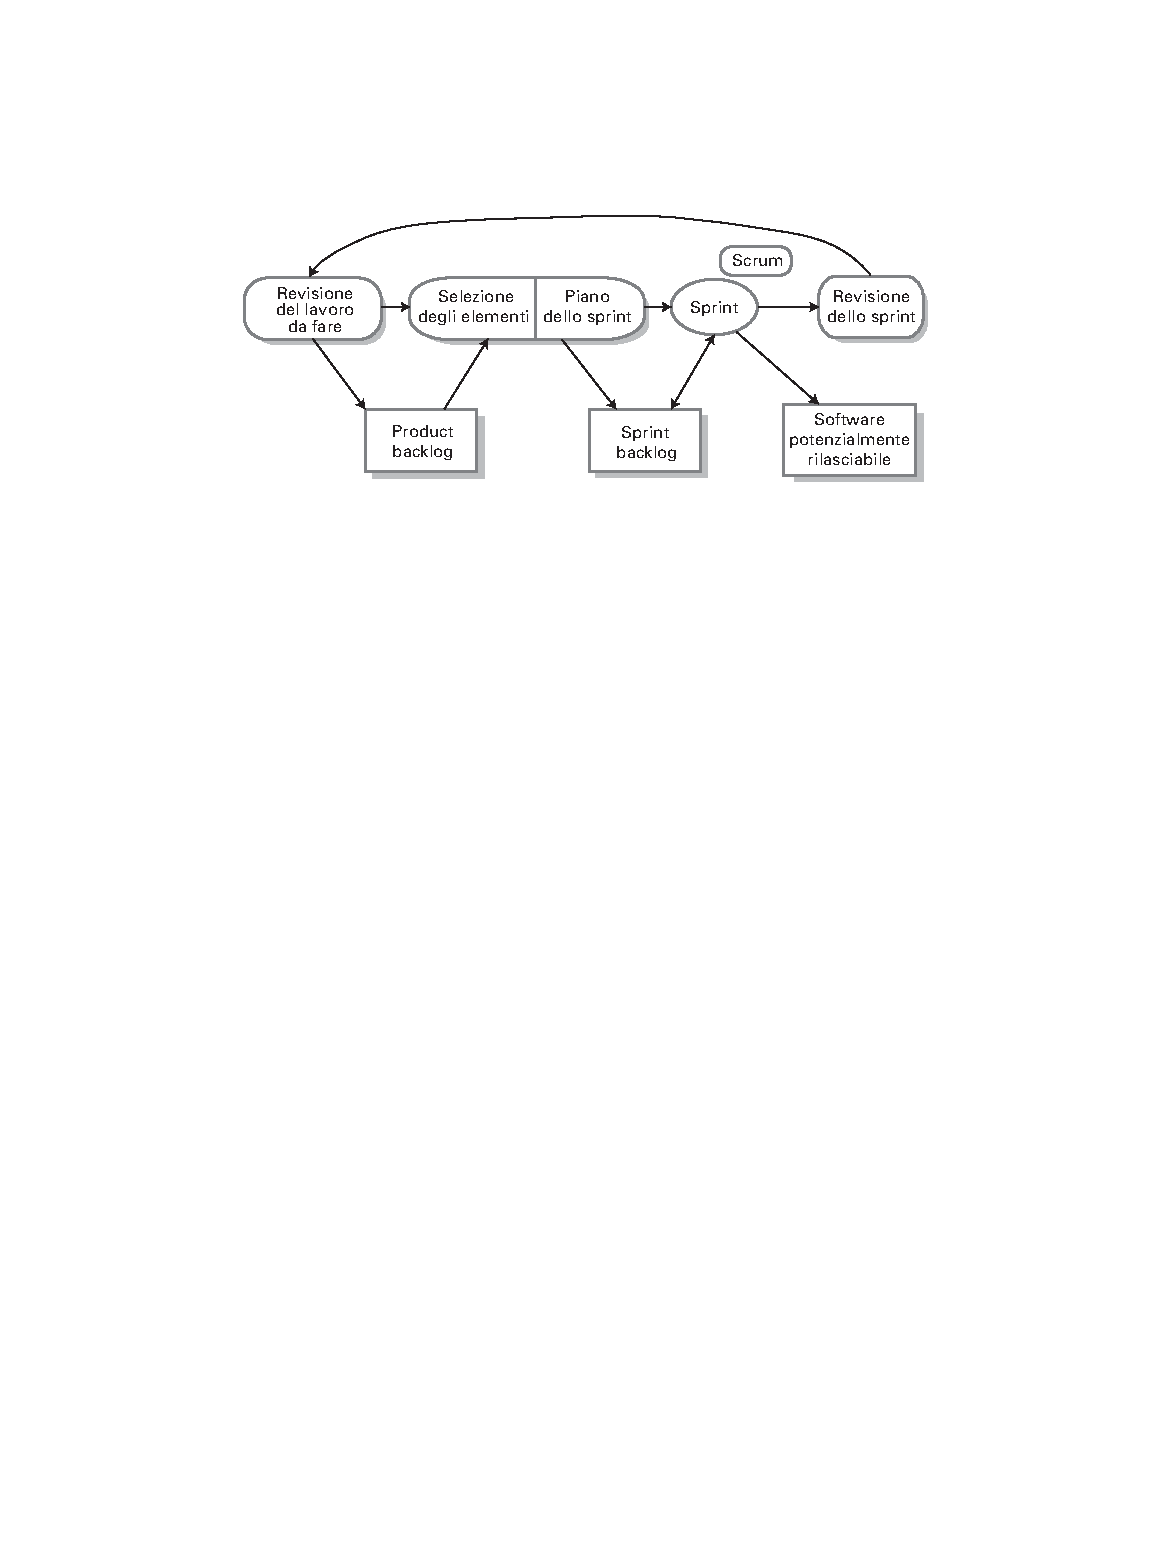
\includegraphics[width=0.9\textwidth]{diagrams/scrum.pdf}
	\caption{Activity Diagram - Metodo Scrum}
	\label{fig:scrum}
\end{figure}
\newpage
In alcuni casi, sono state effettuate sessioni di \textbf{\emph{pair programming}} (programmazione a coppie), in cui i membri del team si incontravano per migliorare il software o creare parti di documentazione.




\newpage
\subsection{Progettazione architetturale e pattern utilizzato}
Il sistema è stato sviluppato utilizzando le tecniche di modellazione ad oggetti.\\
\\Per facilitare lo sviluppo, è stato scelto il pattern architetturale \textbf{\emph{MVC}}, dividendo però tra più classi i compiti di ciascun componente seguendo la filosofia del \emph{divide et impera}. La suddivisione dei componenti in classe, successivamente approfondita nel \textbf{\emph{Class Diagram}}, è la seguente:
\begin{itemize}
	\item \textbf{Model}: Si occupa di gestire i dati utilizzati dall'applicazione. Nel progetto è costituito dalla classe Business, un singleton rappresentante l'agenzia che si occupa di fornire il servizio di gestione dei lavoratori. Contiene tutti i dati inerenti ai responsabili e lavoratori registrati, insieme a tutti i metodi necessari alla gestione di questi. La memorizzazione dei dati è implementata tramite serializzazione.
	\item \textbf{View}: Si occupa della visualizzazione dei dati sull'interfaccia utente e della creazione e gestione di quest'ultima. Nel progetto è costituita dalle classi Window, SceneBuilder e Popup. Le classi Window sono implementate seguendo il factory pattern e si occupano di creare una nuova finestra, chiamando i metodi di SceneBuilder per posizionare i vari campi e pulsanti. Le classi Popup, anch'esse un factory pattern, si occupano della creazione di una finestra popup per dare messaggi di errore, avviso o successo all'utente.
	\item \textbf{Controller}: Si occupa di ricevere tramite l'interfaccia gli input dell'utente e dopo averli elaborati li converte in comandi per Model e View. Nel progetto è costituito dalla classe Events e dalle classi che contengono i dati di lavoratori e responsabili. Queste ultime si occupano, quando viene chiamato il loro costruttore, di controllare i dati passati in input dall'utente, lanciando un'eccezione con messaggio in caso di dati non validi. Le eccezioni vengono poi fermate così che il componente View possa mostrare a schermo un popup di errore con il messaggio dell'eccezione. La classe Events invece contiene i metodi che assegnano ad un pulsante il proprio comportamento, come ad esempio prelevare i dati inseriti dall'utente.
\end{itemize}

\newpage

\subsection{Class Diagram}

\begin{figure}[htpb]
	\centering
	\hspace*{-2cm}
	\vspace*{-0.5cm}
	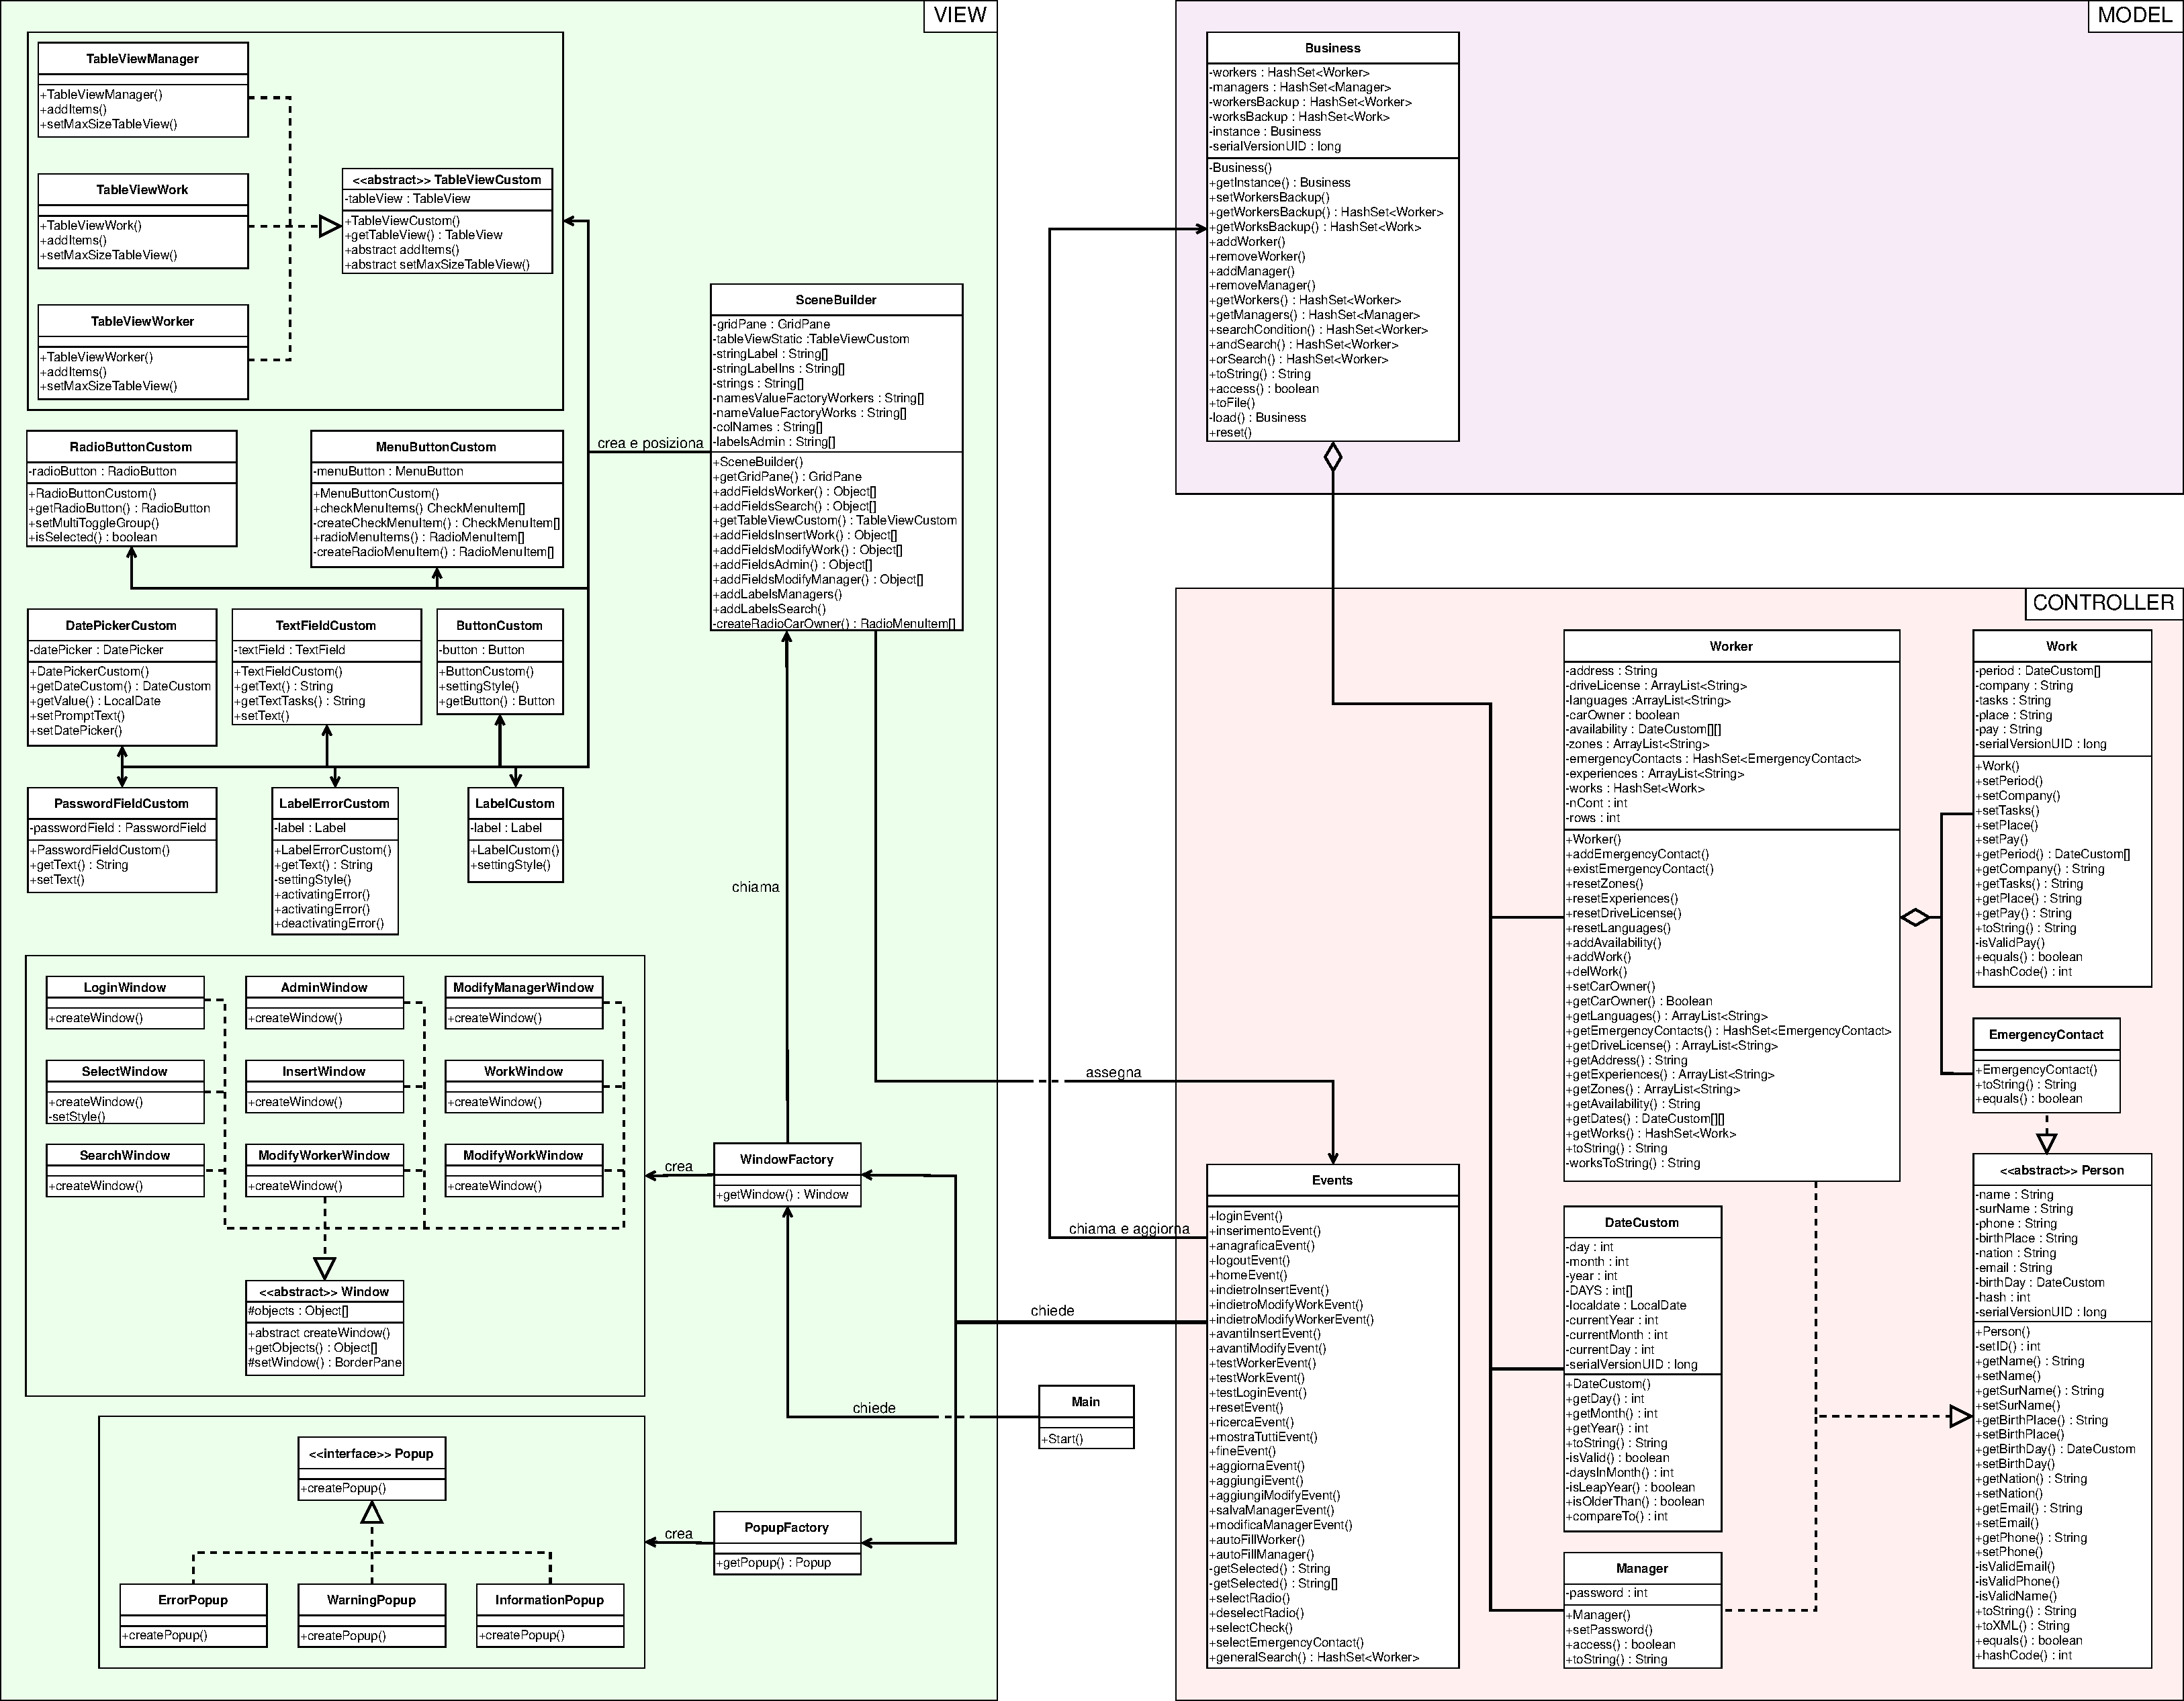
\includegraphics[width=1.3\textwidth]{diagrams/Class_Diagram_Vertical.pdf}
	\label{fig:cls_dia}
\end{figure}

\subsection{Design pattern}
\begin{itemize}
	\item \textbf{Pattern Singleton}: Il \emph{Singleton} è utilizzato per
	assicurare l'esistenza di una ed unica istanza di un oggetto con un punto di accesso comune. Nel progetto è stato utilizzato per la classe \emph{Business} in quanto questo ne rende più comodo l'accesso, semplificando e rafforzando la sicurezza del sistema di salvataggio tramite serializzazione.
	\item \textbf{Pattern Factory}: Questo pattern è utilizzato per non esporre al client le logiche e i metodi di creazione degli oggetti permettendo però di utilizzare un'interfaccia comune per riferirsi ad essi. In questo caso è stato utilizzato in maniera piuttosto estensiva per la creazione delle classi \emph{Popup} e per le classi \emph{Window}, che si occupano di creare tutte le finestre grafiche dell'applicazione.
\end{itemize}

\newpage

\subsection{Sequence Diagram del software progettato}

Seguono i Sequence Diagram del software. Sono state riportate, seppur in modo sufficientemente dettagliato, solo le interazioni più importanti.\\
Si noti che tutte le classi di tipo \emph{Window} sono chiuse poco dopo la creazione, senza ulteriori scambi di dati, questo perché si occupano di posizionare finestra e campi sullo stage passato come parametro, una volta ottenuti i campi appena posizionati sulla finestra non vengono più richiamate.\\
Sono inoltre stati omessi, per semplificare i diagrammi, eventuali loop che indichino la ripetibilità di un'azione da parte dell'utente. I diagrammi mostrano quindi una semplice sequenza con le singole possibili scelte dell'utente.\\
\\

\begin{figure}[htpb]
	\centering
	\hspace*{-2cm}
	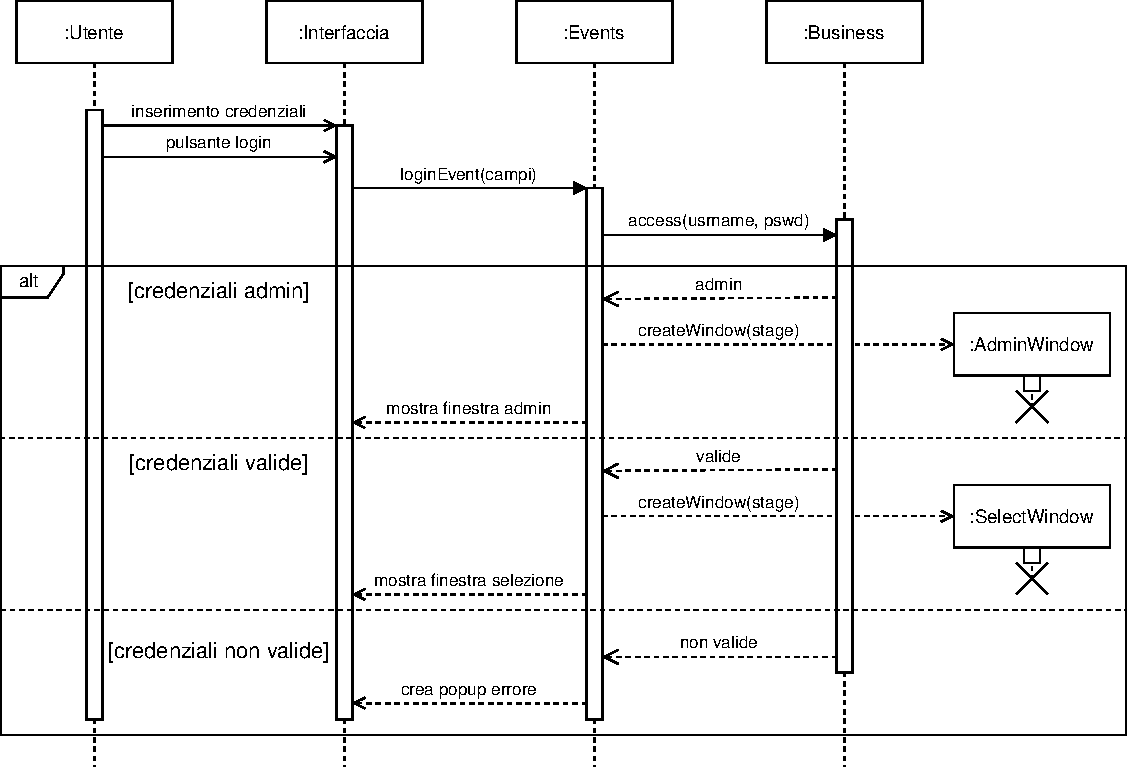
\includegraphics[width=1.3\textwidth]{diagrams/Sequence_Diagram_-_Login.pdf}
	\caption{Sequence Diagram - Login di admin e responsabile}
	\label{fig:sqc_dia_log}
\end{figure}

\begin{figure}[htpb]
	\centering
	\hspace*{-2cm}
	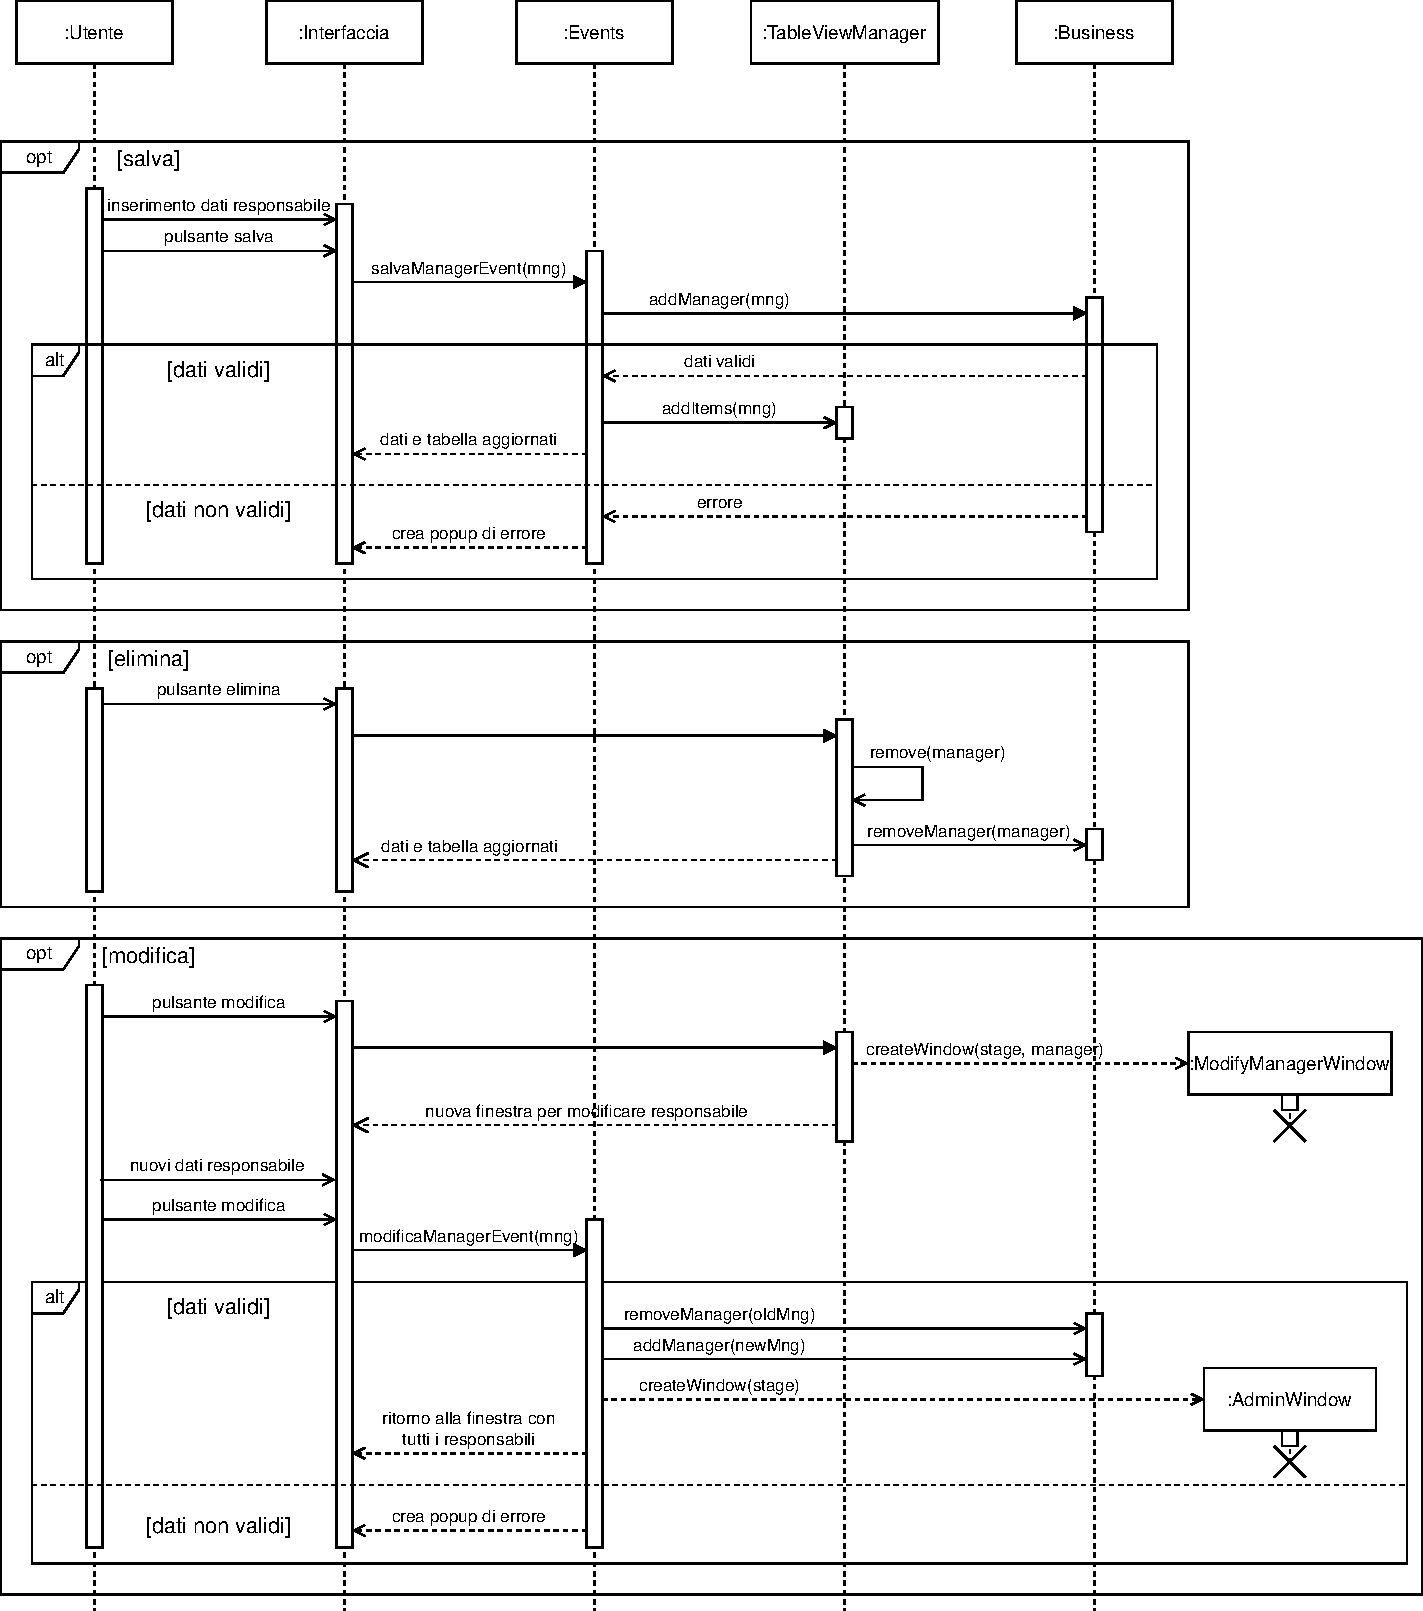
\includegraphics[width=1.3\textwidth]{diagrams/Sequence_Diagram_-_Managers.pdf}
	\caption{Sequence Diagram - Gestione dei responsabili}
	\label{fig:sqc_dia_man}
\end{figure}

\begin{figure}[htpb]
	\centering
	\hspace*{-2cm}
	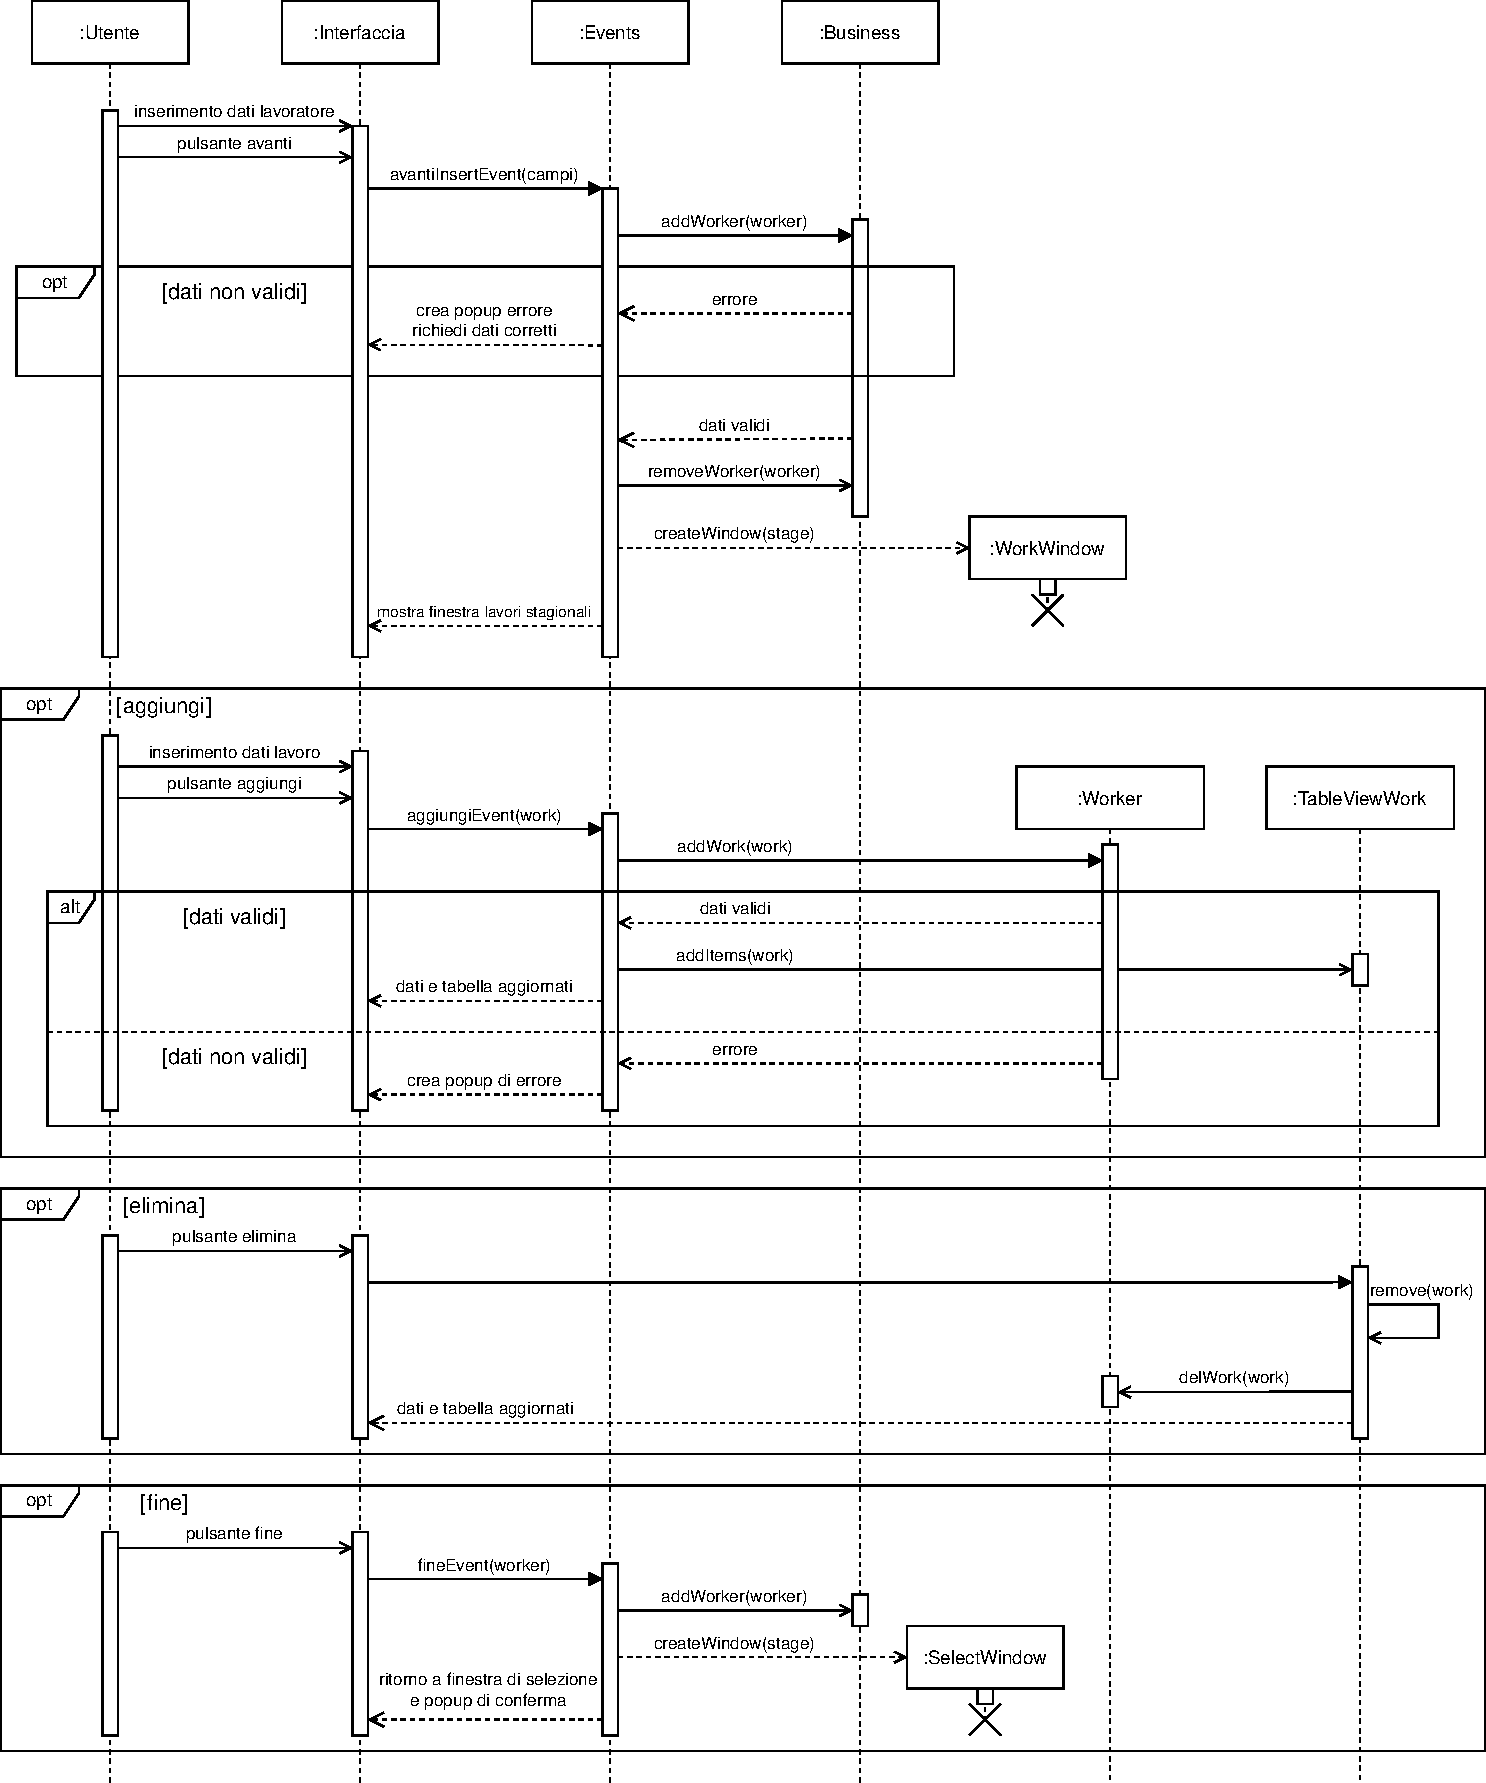
\includegraphics[width=1.3\textwidth]{diagrams/Sequence_Diagram_-_Inserimento.pdf}
	\caption{Sequence Diagram - Inserimento di un lavoratore e dei suoi lavori stagionali}
	\label{fig:sqc_dia_ins}
\end{figure}

\begin{figure}[htpb]
	\centering
	\hspace*{-2cm}
	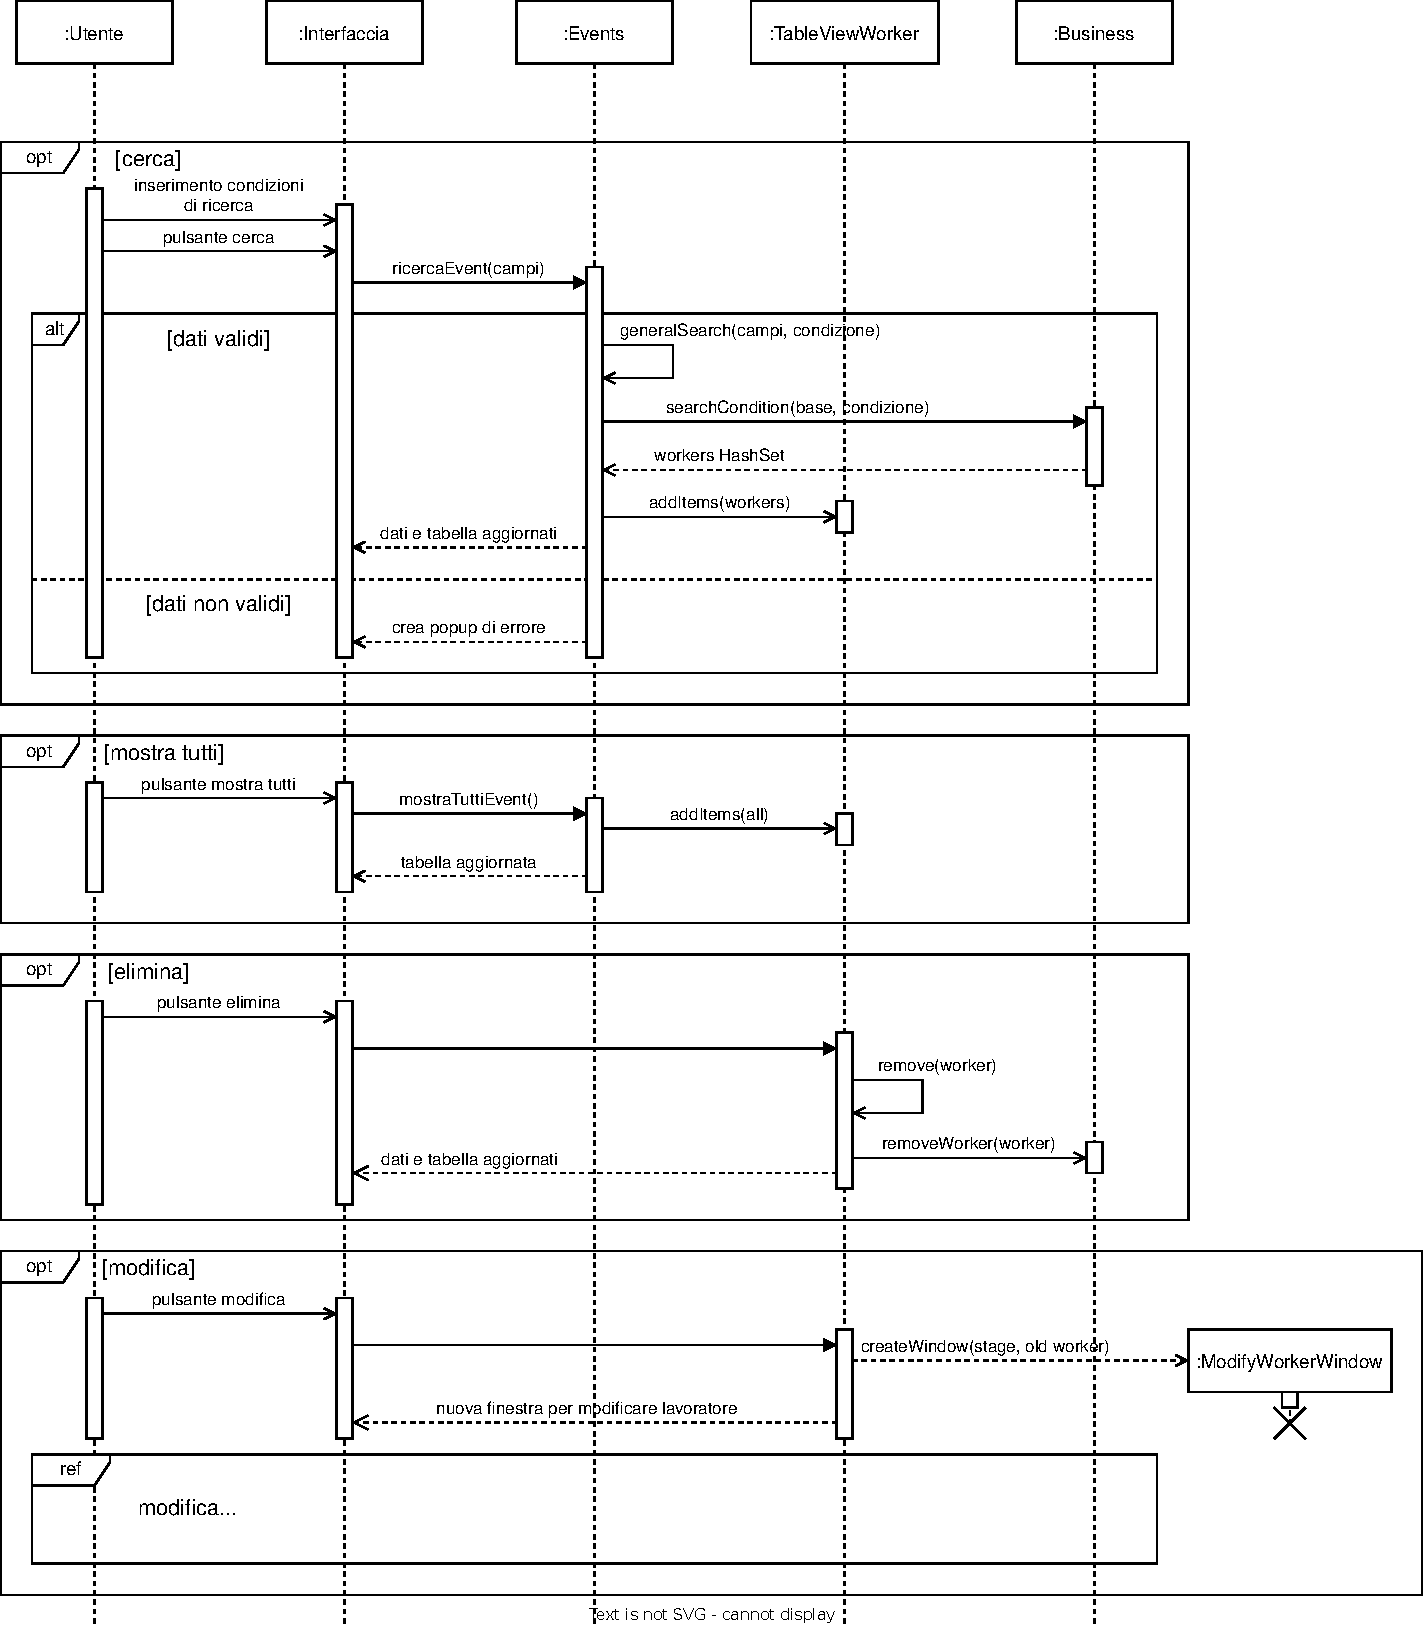
\includegraphics[width=1.3\textwidth]{diagrams/Sequence_Diagram_-_Ricerca.pdf}
	\caption{Sequence Diagram - Ricerca e visualizzazione dei lavoratori}
	\label{fig:sqc_dia_src}
\end{figure}

\begin{figure}[htpb]
	\centering
	\hspace*{-2cm}
	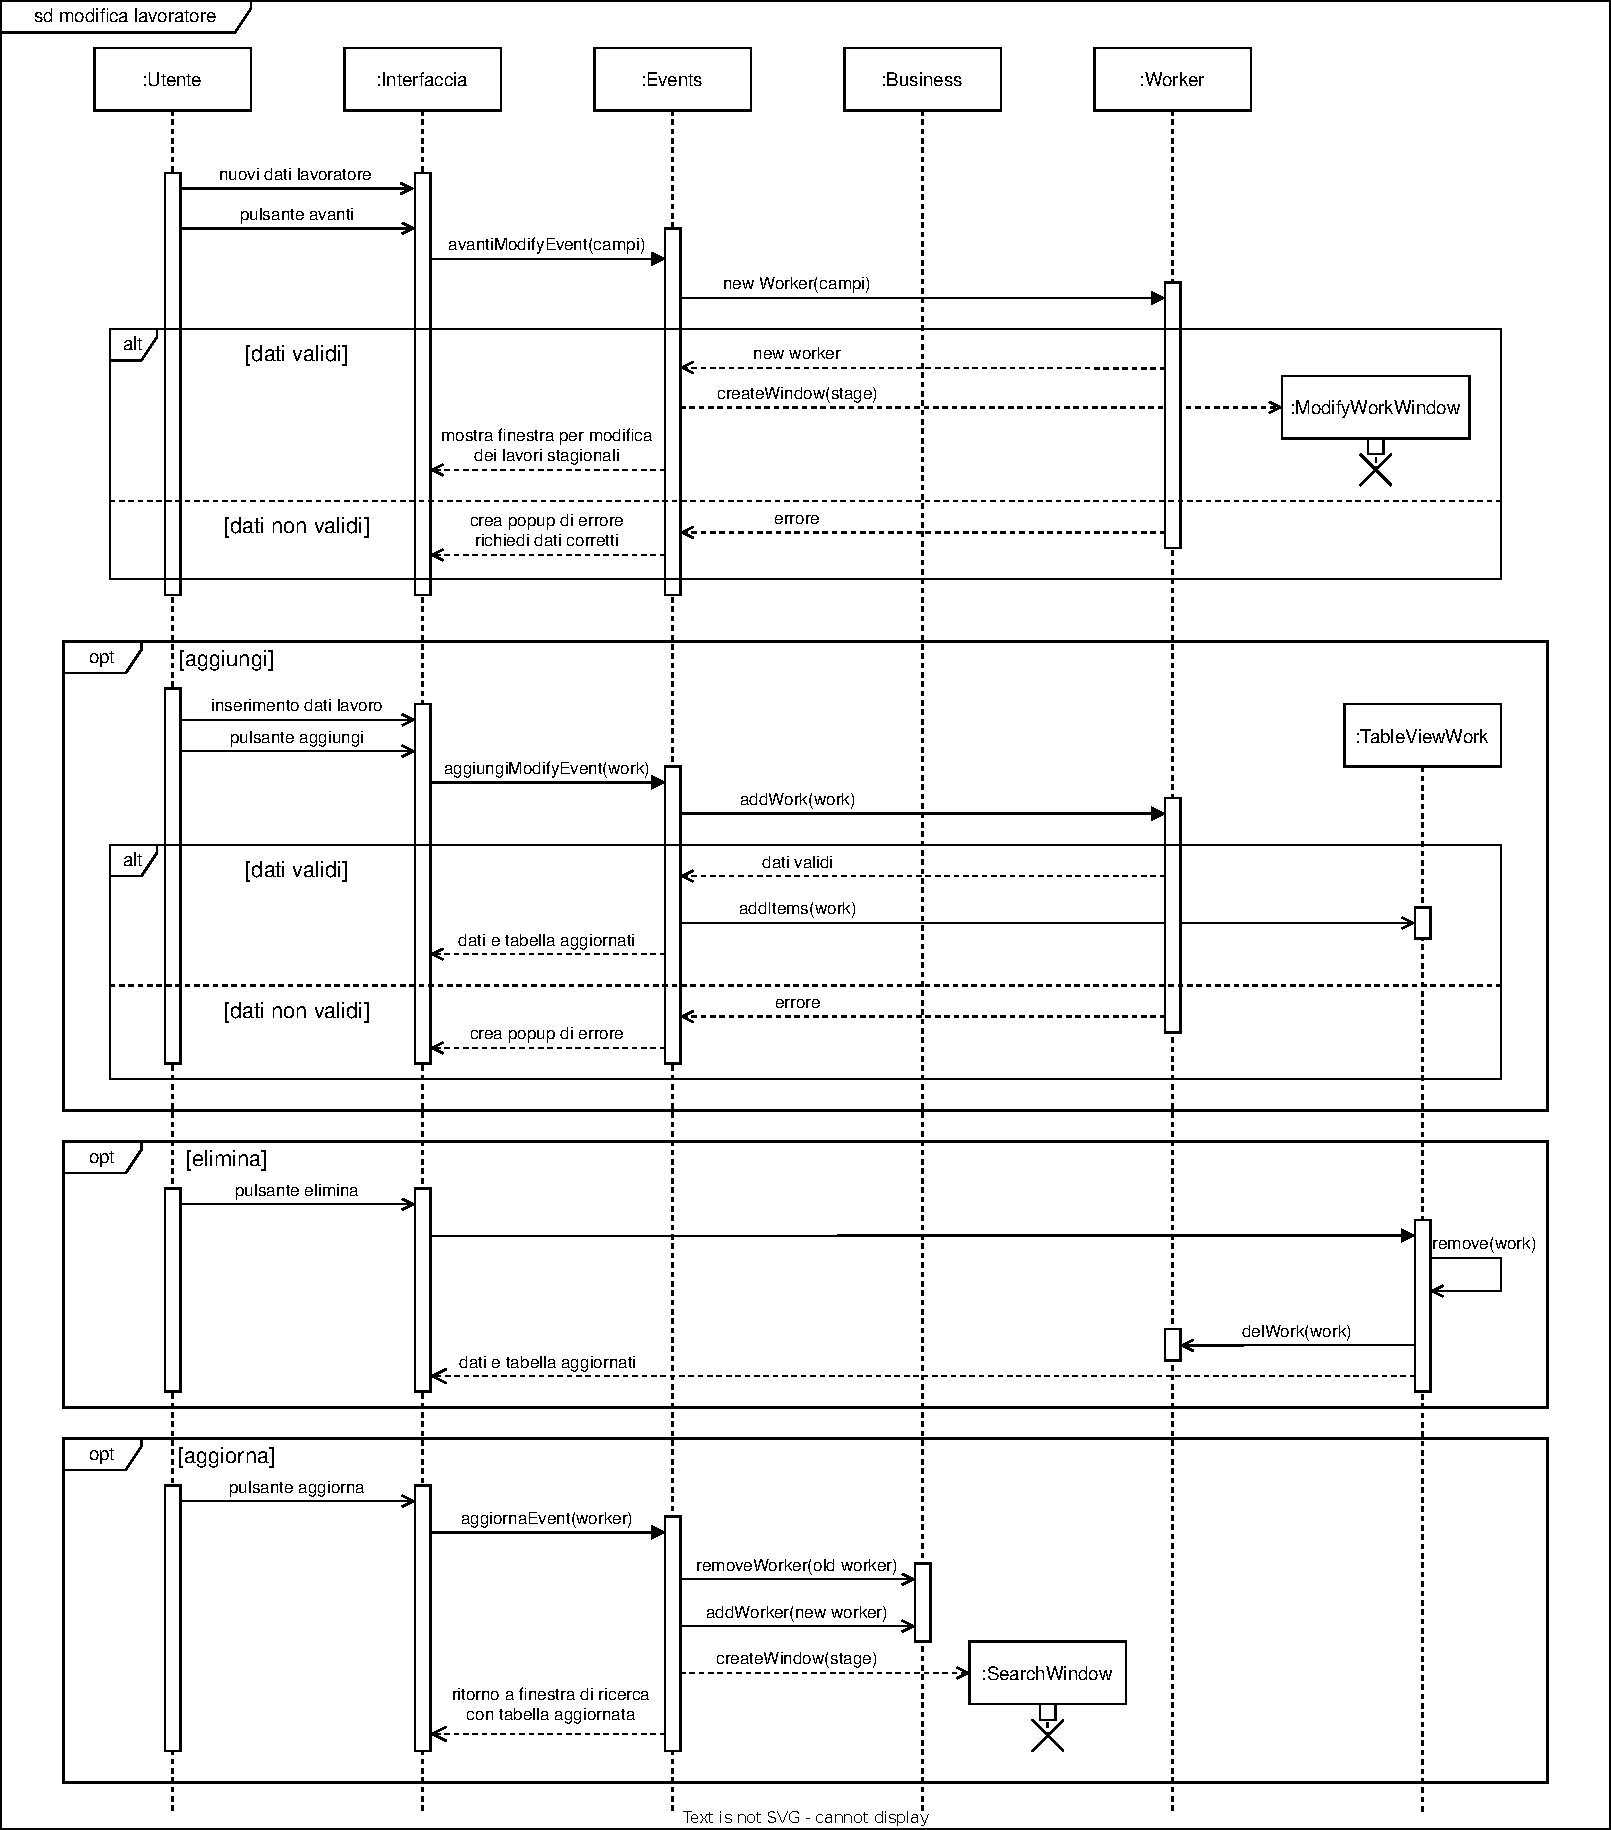
\includegraphics[width=1.3\textwidth]{diagrams/Sequence_Diagram_-_Modifca_lavoratore.pdf}
	\caption{Sequence Diagram - Modifica di un lavoratore e dei suoi lavori stagionali}
	\label{fig:sqc_dia_mod}
\end{figure}

\newpage

\section{Test sul sistema}
Il sistema è stato scrupolosamente sfruttato ad ogni rilascio di versione e
dopo ogni completamento di task da parte dei programmatori. Da notare che i test
sono stati in primo luogo effettuati internamente al termine di ogni nuova
implementazione, in seguito all'unione delle varie parti di codice completate
dal team e poi insieme al cliente. Quest'ultimo ha suggerito di volta in volta
eventuali nuove revisioni di funzionalità inserite e quelle da aggiungere al
sistema in base ai suoi bisogni.\\
Una volta raggiunta l'approvazione del cliente si è proceduto al
successivo ciclo di sviluppo e all'implementazione delle funzionalità
successive.\\
Il ciclo di test prevede, oltre ai controlli di qualità e funzionalità
standard, un approfondito ciclo di \emph{Unit test} in modo da assicurare il
funzionamento corretto delle singole componenti prima dell'unione al software
unitario così da accelerare i tempi di presentazione al cliente.\\
Il cliente infine ha il compito di verificare, tramite utilizzo standard e con
configurazioni particolari, eventuali situazioni non previste dagli sviluppatori
o errori non catturati dai quality assesment effettuati internamente.

\newpage

\subsection{Test eseguiti dagli sviluppatori}
Di seguito una lista comprensiva delle verifiche effettuate dagli sviluppatori sugli input inseribili nel programma e la capacità di questo nel riceverli e gestirli:
\begin{itemize}
	\item \textbf{Verifica di impossibilità di accesso da parte di un utente non autorizzato}
	\item \textbf{Salvataggio dei dati}
	\item \textbf{Eliminazione del salvataggio ed esecuzione del programma "a vuoto"}
	\item \textbf{Verifica della validità nell'inserimento di nome e cognome}: Nello specifico che non ci siano numeri o caratteri speciali inseriti
	\item \textbf{Verifica della validità del numero di telefono}: Il valore inserito deve essere esclusivamente numerico
	\item \textbf{Verifica della validità delle date}: Non deve essere possibile inserire date arbitrare, i periodi di inizio e fine validità devono essere coerenti, se una data si riferisce al giorno corrente e questa viene scritta nel passato non deve essere valida (caso del periodo di fine disponibilità da parte del lavoratore)
	\item \textbf{Verifica di validità dell'inserimento di una mail}
	\item \textbf{Impossibilità di lasciari incompleti i campi obbligatori}
	\item \textbf{Funzionalità corretta della funzione di ricerca}: Correttezza nelle ricerche utilizzando vari operatori di ricerca AND e OR, ricerche parziali completando solo alcuni dei campi disponibili.
	\item \textbf{Modifica ed eliminazione dei valori}: Valido per tutti gli oggetti inseriti che lo prevedono, come i lavori stagionali e i lavoratori, controllare che l'autocompletamento dei campi nelle interfacce di modifica avvenga con successo, così come l'eliminazione degli oggetti che deve avvenire in maniera puntuale, corretta e senza errori
	\item \textbf{Possibilità di navigazione a ritroso delle finestre}: Dove previsto, tornare indietro alla finestra precedente deve conservare correttamente i dati inseriti e la navigazione deve avvenire puntualmente secondo l'ordine stabilito e senza errori.
	\item \textbf{Verifica del salvataggio con chiusura}: alla chiusura del programma, da qualsiasi punto, tutti i dati confermati dall'utente devono essere salvati senza errori e recuperati correttamente al riavvio. 
\end{itemize}

\end{document}